%% ----------------------------------------------------------------
%% Thesis.tex -- MAIN FILE (the one that you compile with LaTeX)
%% ---------------------------------------------------------------- 

% Set up the document
\documentclass[a4paper, 11pt, oneside]{Thesis}  % Use the "Thesis" style, based on the ECS Thesis style by Steve Gunn
\graphicspath{Figures/}  % Location of the graphics files (set up for graphics to be in PDF format)

% Include any extra LaTeX packages required
%\usepackage[square, numbers, comma, sort&compress]{natbib}  % Use the "Natbib" style for the references in the Bibliography
\usepackage[authoryear]{natbib}%for author year citations

\usepackage{verbatim}  % Needed for the "comment" environment to make LaTeX comments
\usepackage{vector}  % Allows "\bvec{}" and "\buvec{}" for "blackboard" style bold vectors in maths
\hypersetup{urlcolor=blue, colorlinks=false}  % Colours hyperlinks in blue, but this can be distracting if there are many links.
\usepackage{fontspec}
\usepackage{xeCJK} % Japanese support
\usepackage{longtable}
\setCJKmainfont{Noto Serif CJK JP}

%import my data
%%%%%%%%%%%%%%%%%%%%%%%%%%%%%%%%%%%%%%%%%%%%%%%%%
%
%       Data for Title Page
%                
%
%%%%%%%%%%%%%%%%%%%%%%%%%%%%%%%%%%%%%%%%%%%%%%%%%

\newcommand{\authorname}{Megan Horikawa} % Name

\newcommand{\mnr}{6196282} % Matrikelnummer, bspw.: 12345

\newcommand{\betreuerI}{Prof. Dr. Detmar Meurers} % Name 1. Betreuer bzw. betreuender Prof

\newcommand{\betreuerII}{Prof. Dr. ??? ?} % Name 2. Betreuer
\newcommand{\betreuerIItaetigkeit}{Second Examiner} % Tätigkeit des Betreuers: Fachbetreuer, Wissenschaftlicher Betreuer, Betrieblicher Betreuer

\newcommand{\abschluss}{Master of Arts} % Art des Studiengangs/Abschlusses: Bachelor oder Master
\newcommand{\art}{Masterarbeit} % Art der Arbeit: Projektarbeit, Bachelorarbeit oder Masterarbeit

\newcommand{\zeitraum}{März 2025 -- Juli 2025} % Monat JJJJ -- Monat JJJJ

\newcommand{\thesistitle}{Modeling Proficiency in L2 Japanese: Evaluating linguistic Complexity Measures and Illustrative Features} % Titel der Arbeit

\newcommand{\gebdatum}{12.\,01.\,1990} % Geburtsdatum, TT.\,MM.\,JJJJ

\newcommand{\gebort}{Port Huron, Mi, USA} % Geburtsort

\newcommand{\datum}{01.\,12.\,2025} % z.B. Abgabedatum

% Fakultät und Studiengang:

\newcommand{\fak}{Seminar für Sprachwissenschaft} % Eingabe der Fakultät
\newcommand{\studiengang}{International Studies in Computational Linguistics} % Eingabe des Studiengangs
\title{}
\authors{}
%% ----------------------------------------------------------------
\begin{document}
\frontmatter      % Begin Roman style (i, ii, iii, iv...) page numbering

% Set up the Title Page
%\title  {Thesis Title}
%\authors  {\texorpdfstring
%            {\href{your web site or email address}{Megan Horikawa}}
%            {Author Name}
%            }
%\addresses  {\groupname\\\deptname\\\univname}  % Do not change this here, instead these must be set in the "Thesis.cls" file, please look through it instead

%\date       {\today}
%\subject    {Computational Linguistics}
%\keywords   {}

%using a different title page:

%%%%%%%%%%%%%%%%%%%%%%%%%%%%
%   Title Page
%%%%%%%%%%%%%%%%%%%%%%%%%%%%
\begin{titlepage}
{\centering
{\Large \textbf{Eberhard Karls Universität Tübingen}\par}
{\large \textbf{Philosophische Fakultät \fak} \par}
{\large \abschluss-\studiengang\par}
\vspace{1.75cm}
{\Large \textbf{\thesistitle}\par}
\vspace{1.5cm}
{\large \art \par}
\vspace{3cm}
{\large  von\par}
\vspace{1.25cm}
{\author\\[3ex]
megan.horikawa@student.uni-tuebingen.de\\[3ex]
%\mnr % I don't think I need to include this
\par}}
\vfill
{\noindent First Examiner and Supervisor: \betreuerI 
\par \vspace{0.25cm}
\betreuerIItaetigkeit: \betreuerII
\par \vspace{0.75cm}
Tübingen, \zeitraum} % ggf. Ort anpassen
\end{titlepage}


%% ----------------------------------------------------------------

\setstretch{1.3}  % It is better to have smaller font and larger line spacing than the other way round

% Define the page headers using the FancyHdr package and set up for one-sided printing
\fancyhead{}  % Clears all page headers and footers
\rhead{\thepage}  % Sets the right side header to show the page number
\lhead{}  % Clears the left side page header

\pagestyle{fancy}  % Finally, use the "fancy" page style to implement the FancyHdr headers


%%%%%%%%%%%%%%%%%%%%%%%%%%%%
%   Authorship Declaration
%%%%%%%%%%%%%%%%%%%%%%%%%%%%
 % Declaration Page required for the Thesis, your institution may give you a different text to place here
\Declaration{

\addtocontents{toc}{\vspace{1em}}  % Add a gap in the Contents, for aesthetics

Ich erkläre hiermit, dass ich die vorliegende Arbeit selbständig verfasst habe, dass
ich keine anderen als die angegebenen Hilfsmittel und Quellen benutzt habe, dass
ich alle wörtlich oder sinngemäß aus anderen Werken \"ubernommenen Aussagen als
solche gekennzeichnet habe, dass die Arbeit weder vollständig noch in wesentlichen
Teilen Gegenstand eines anderen Pr\"ufungsverfahrens gewesen ist, dass ich die Arbeit
weder vollständig noch in wesentlichen Teilen bereits veröffentlicht habe, und
dass das in Dateiform eingereichte Exemplar mit dem eingereichten gebundenen
Exemplar \"ubereinstimmt.\\


\begin{tabular}{@{}p{.5in}p{4in}@{}}
Signed: & \hrulefill \\
& \textit{(Megan Horikawa)} \\
\end{tabular}
 
}
\clearpage 
 
%%%%%%%%%%%%%%%%%%%%%%%%%%%%
%   Quote Page % not sure I really need this
%%%%%%%%%%%%%%%%%%%%%%%%%%%%
% The "Funny Quote Page"
\pagestyle{empty}  % No headers or footers for the following pages

\null\vfill
% Now comes the "Funny Quote", written in italics
\textit{``Write a funny quote here.''}

\begin{flushright}
If the quote is taken from someone, their name goes here
\end{flushright}

\vfill\vfill\vfill\vfill\vfill\vfill\null
\clearpage  % Funny Quote page ended, start a new page
%% ----------------------------------------------------------------

%%%%%%%%%%%%%%%%%%%%%%%%%%%%
%   Abstract
%%%%%%%%%%%%%%%%%%%%%%%%%%%%
% The Abstract Page
\addtotoc{Abstract}  % Add the "Abstract" page entry to the Contents
\abstract{
\addtocontents{toc}{\vspace{1em}}  % Add a gap in the Contents, for aesthetics

This study investigates the use of linguistic complexity features to model proficiency levels in Japanese as a second language (L2). Drawing on a corpus of learner essays, the research examines whether linguistic complexity, and/or criterial features can reliably reflect L2 development and support interpretable proficiency classification. An Explainable Boosting Machine (EBM) was used to model the relationship between these features and proficiency labels, offering transparency in identifying which linguistic measures constribute most to level prediction.

The model achieved 38\% accuracy in five-class classification, well above the baseline.  Feature importance analysis revealed that mainly linguistic complexity measures such as, coordinate clauses per sentence, Morphological Complexity Index, and Lexical Frequency profiles were key predictors, although one criterial feature, passive form, was also ranked in the top 15 features. These findings align with established theories that linguistic complexity increases with proficiency, though unexpected trends-such as early subordination and continued growth in coordination-suggest the influence of instruction sequences and parser limitations.

Beyond modeling, the study also highlights developmental trajectories in complexity measures and discusses implications for language assessment, curriculum design, and learner feedback. Limitations include the use of uncorrected learner data, reliance on surface-form features, and imbalanced class sizes, especially for N1 learners. Future work can explore error-based features, discourse-level complexity, and longitudinal data collection. This research contributes to both second language acquisition theory and the development of computational tools for assessing L2 Japanese proficiency.
}

\clearpage 


\setstretch{1.3}  % Reset the line-spacing to 1.3 for body text (if it has changed)

%%%%%%%%%%%%%%%%%%%%%%%%%%%%
%   Acknowledgements
%%%%%%%%%%%%%%%%%%%%%%%%%%%%

\acknowledgements{
\addtocontents{toc}{\vspace{1em}}  % Add a gap in the Contents, for aesthetics

The acknowledgments and the people to thank go here, don't forget to include your project advisor\ldots
\begin{itemize}
    \item Dr. Detmar Meurers
    \item Dr. Xiaobin Chen & kibi team
    \item Dr. Mutsuko Endo-Hudson
    \item Family
\end{itemize}
}
\clearpage

\pagestyle{fancy}  %The page style headers have been "empty" all this time, now use the "fancy" headers as defined before to bring them back


%% ----------------------------------------------------------------
\lhead{\emph{Contents}}  % Set the left side page header to "Contents"
\tableofcontents  % Write out the Table of Contents

%% ----------------------------------------------------------------
\lhead{\emph{List of Figures}}  % Set the left side page header to "List if Figures"
\listoffigures  % Write out the List of Figures

%% ----------------------------------------------------------------
\lhead{\emph{List of Tables}}  % Set the left side page header to "List of Tables"
\listoftables  % Write out the List of Tables

%% ----------------------------------------------------------------
\setstretch{1.5}  % Set the line spacing to 1.5, this makes the following tables easier to read
\clearpage  % Start a new page


% End of the pre-able, contents and lists of things

%%%%%%%%%%%%%%%%%%%%%%%%%%%%%%%%%%%%%
% Dedication Page?
%%%%%%%%%%%%%%%%%%%%%%%%%%%%%%%%%%%%%

%% Begin the Dedication page

\setstretch{1.3}  % Return the line spacing back to 1.3

\pagestyle{empty}  % Page style needs to be empty for this page
\dedicatory{For/Dedicated to/To my\ldots}
\begin{itemize}
    \item Dr. Detmar Meurers
    \item Dr. Xiaobin Chen & kibi team
    \item Dr. Mutsuko Endo-Hudson
    \item Family
\end{itemize}
\addtocontents{toc}{\vspace{2em}}  % Add a gap in the Contents, for aesthetics
 later....


%% ----------------------------------------------------------------
\mainmatter	  % Begin normal, numeric (1,2,3...) page numbering
\pagestyle{fancy}  % Return the page headers back to the "fancy" style

% Include the chapters of the thesis, as separate files
% Just uncomment the lines as you write the chapters

\chapter{Introduction}

%Motivation for what I am trying to do....Language proficiency classification and which measures are reliably able to classify proficiency - automated scoring/grading of tests. etc. using linguistic complexity measures.

%Train classification models using complexity features.... which features perform
%better?

% Why does this matter?
% - addressing a gap in research for Japanese
% - Evaluating language development/proficentcy levels in SLA
% - can automatically evaluate a lerner's proficentcy level

%Define problem:
% Many measures do the measures vary across languages?
%Focus of indo-european languages and English, not much info on Japanese
% unclear methods of measure,


% can help inform instructional design of Japanese material?
% automated proficentcy testing?

% complexity studies have differed in their findings....and definitions of what complexity is have also been varried
% and vague
% developmental tradjectory of L2 Japanese - using traditional complexity measures and also sophistication measures
% (frequency of certain forms)

Language learners' proficiency in their target language is typically assesed using established frameworks such as the \textbf{Common European Framework of Reference for Languages (CEFR)}, and the \textbf{American Council on the Teaching of Foreign Languages (ACTFL)}. These frameworks define proficiency levels using generalized "can-do" statements, which help standardize assessment across multiple languages.  However, because they are designed for broad applicabiliy, these frameworks may not fully capture language-specific developmental patterns, particularly in languages which significantly differ from Indo-European languages.

In second language acquisition (SLA) research, proficiency is often analyzed in terms of three core
domains:complexity, fluency, and accuracy \cite(Skehan1989). of these, complexity has been the subject of extensive
investigation, particularly in written languages, where it serves as an indicator of linguistic development
\cite(Lu2010, Lu2011, Ortega2003, Iwashita2006). Complexity measures, including syntactic, and lexical features have
been widely used to evaluate proficency, yet findings across studies have varied significantly. This inconsistency
has been attributed to differences in how complexity is defined, how it is measured, or how the tasks influence
outcomes \cite(Butle2012). Many linguistic complexity measures have been proposed, but their effectiveness has
varied among studies. In L2 Japanese research, there is limited empirical evidence on which complexity measures best predict proficiency.

While much of this research has focused on English and Indo-European languages, fewer studies have explored how
complexity develops in Japanese as a second language (JSL). Given that Japanese differs typologically from
Indo-European languages in aspects such as morphology, syntax, and even orthography, it is unclear whether
complexity measures that work well for English apply equally to Japanese. Examining linguistic complexity in L2
Japanese learners can provide new insights into second language development and help refine assessment methods.

Moreover, automated scoring and evaluation systems increasingly rely on linguistic complexity measures to classify
proficiency levels. However, without a clear understanding of which complextiy features best differenticate between
proficiency levels in Japanese, automated systems may lack accuracy and interpretability. Addressing this gap can
contribute to more effective automated proficiency assessment and inform the design of instructional materials
tailored towards learners of Japanese.

In this thesis I aim to  investigate how linguistic complexity develops in L2 Japanese learners by analyzing
both traditional syntactic and lexical complexity measures and sophistication measures (such as frequency-based
indicators of linguistic structures). Understanding these developmental patterns can provide a more nuanced
perspective on SLA trajectories in Japanese and constribute to automated proficiency classification models. Within
this thesis I will address the following:
\begin{enumerate}
    \item To identify which syntactic complexity measures show reliability as indices of language development in
    L2 Japanese learners.% Which syntactic complexity measures show reliability as indices for languagedevelopment/proficiency level?
    \item To examine how linguistic complexity features develop across different proficency levels in Japanese
    learners.
    %How do linguistic complexity features develop across different proficiency levels in Japanese as a second language learners?
    \item To analyze the influence of a learner's first language (L1) on the developmental trajectory of Japanese
    complexity features.
    %What influence does a learner's L1 have on their developmental tradjectory of Japanese
    \item To assess whether linguistic complexity features can reliably predict proficiency levels in L2 Japanese
    learners.
    %Can linguistic complexity features reliably predict proficiency levels in Japanese second language learners?
\end{enumerate}

This thesis is structured as follows: \textbf{chapter 2} provides background on linguistic complexity, including an
overview of complexity measures and their role in SLA research.
\textbf{Chapter 3} outlines the research methodology, detailing the learner corpus, and calculation of the complexity
measures chosen.
 \textbf{Chapter 4} presents an evaluation of initial findings, including how complextiy features develop across
proficiency levels.
\textbf{Chapter 5 }will present my findings and results of classification models, while \textbf{Chapter 6}
discusses my findings and their implications for SLA research and automated proficiency assessment, and directions for
future research. % Introduction

\chapter{Background/Related Work}
%What do I need to know to understand the approach described in the methodology section?

\section{Linguistic Complexity}
%-What is complexity? How it is defined? in SLA literature?
%-Distiction between complexity, accuracy, and fluency (CAF Framework).
%- Types of Complexity: Syntactic, lexical, morphological, discourse?
%- Why complexity is a useful proxy for proficiency. (motivate what is being measured)
%- Mention Task effect?

% i need to be more explicit in differentiating complexity from criterial features - as to some it may seem like they
% overlap. Frequency measures used
% in
% Complexity look at elaboration whereas the frequency in criterial features focuses on the appearance at different
% levels as a developmental pattern.

In second language acquisition (SLA) research a learner's proficiency is analyzed through the triad of domains known
as \textbf{complexity}, \textbf{accuracy}, and \textbf{fluency} (CAF) \cite{Skehan1989,ellis2003}. Each of these
dimensions are treated as key indicators of language development in a learner, with each dimension capturing different
aspects of learner performance. \textbf{Accuracy} is concerned with the extent a learner's language conforms with
the norms of the target language, usually measured by an error rate. While this seems clear-cut, there is
controversy regarding the criteria for evaluating and identifying errors and how much they should follow
prescriptive norms of the target language \cite{housen2009}. \textbf{Fluency} focuses on the learner's
speed and smoothness of production, measured by counting the rate of production units. Due to the nature of data
needing a time variable, usually oral data is analyzed for these studies. Finally,
\textbf{complexity} is characterized as the ”the extent to which the language
produced in performing a task is elaborate
and varied" \cite{ellis2003}. Complexity has attracted considerable attention
in studies analysing written language as a proxy for development.

Despite its widespread use, the concept of complexity has been inconsistently defined across studies. Researchers
have introduced more refined distinctions such as, 'absolute vs relative'
complexity
\citet{Miestamo2008, Butle2012}, and
'linguistic' vs. 'cognitive' complexity \cite{housen2009}. In these models, the first term refers to characteristics
of the linguistic system itself (e.g. structural elaboration), including how complex a sentence is in terms of its
syntax (e.g. number of clauses, subordination, embedding) or its vocabulary (e.g., lexical diversity, word frequency)
. These features can be measured objectively from the surface structure of the texts independent of the learner.
Whereas the second terms (relative and cognitive) focused on the processing demand on the learner or reader.
These distinctions attempt to separate complexity as a
property of the language system from the mental effort required to process it.

Further clarifying this divide, \citet{Pallotti2015} argues for distinguishing between complexity, as the formal
characteristics of linguistic structures, and \textbf{difficulty}, which refers to the cognitive demands those
structures place on learners and readers. According to this view, a sentence may be structurally complext but not
necessarily difficult for a proficient speaker, while a relatively simple structure could still pose challenges for
a learner.

 In line with this perspective, this study adopts a dual approach, considering both formal complexity and
difficulty measures as dimensions of learner language. While structural complexity is quantified through
surface-level linguistc features, difficulty is inferred from how these features are likely to affect processing and
comprehension. For instance, in readability research, studies studies such as \citet{Berendes2018}, used a range of
global and local complexity measures to classify german secondary school texts for readability, while
\citet{shain2016}employed syntactic complexity measures using Dependency Locality Theory (DLT) to predict reading
times as a measure of cognitive load. Similarly, \citet{Feng2009} analyzed discourse level features related to
entity density in texts to assess the readability for adults with intellectual disabilities. % add a note that while

In contrast, most SLA studies on learner writing have focused primarily on linguistic complexity as a developmental
marker, using various measures to model language growth
\cite{Lu2010,Lu2011,Vyatkina2012,weiss2019,Iwashita2006,Wolfe1998, Ortega2003,NorrisOrtega2009}. However,
the majority of studies have focused on the domains of syntax and lexical complexity which has been criticized
as \"reductionist\" and too simplistic of an operationalization of linguistic complexity \cite{Butle2012}. In the
following sections below, I
will analyze the different domains of linguistic complexity used in this thesis.

%- Introduce major complexity metrics:
%    -Syntactic: sentence length, clause density, subordination, coordination, noun phrases, dependency distance
%    - Lexical: type-token ratio (TTR), MTLD, lexical sophistication
%-Theoretical basis and interpretation of each measure and limitations
%- Use of NLP tools in measuring complexity and automated tools in ICALL applications (CTAP)

\subsection{Syntactic Complexity}
%- General overview on types of measures
   % - Elaboration:  \citet{Butle2012}
    %- Variation : Diversity of forms and structures
%- introduce measures, especially ones I plan to use information on the calculations should be given in chapter 3 or
%in appendix?

%- both absolute and relative measures included
    %- mean clause length
    %- mean sent length
    %- clauses to sentences ratio (sentence complexity ratio)
    %- Complex NP per sentence
    %- NP per sentence
    %- coordination
    %- subordination
    %- adjective and adverb verb modifiers per VP?
    %- ADD - average dependency distance?

Syntactic complexity  is concerned with quantifying how elaborate and varied the grammatical structures used in a
    text are. A syntactically complex text often contains more structurally rich constructions, resulting in increased length, depth or diversity. Accordingly, measures of syntactic complexity are often divided into those capturing elaboration- referring to the use of
    longer or more embedded structures, and variation, which refers to the range and diversity of syntactic forms
    used.

\citet{Butle2012} further distinguishes syntactic complexity into two dimensions of scale: global and local
measures. Global
measures concern the macro-level structural organization of language or what is described as
\textit{"the size, breadth, width, or richness of the
learner's L2 system"} \cite{Butle2012}. These measures are typically operationalized at the sentence or clause level
and include metrics such as mean length of T-unit/sentence, clauses per T-unit/sentence or complex.They reflect
learner's ability to coordinate and embed clauses into hierarchically structured sentences.

In contrast, the local level addresses more fine-grained measures by analyzing
the internal structure at the phrase or clause level. Measures such as length of noun phrases,
modifiers per noun phrase, and Mean hierarchical distance (MHD) are used to analyze the internal structure and depth
at a more granular level. These local measures capture how syntactic elements are constructed and nested within
smaller constituents, such as within noun or verb phrases, providing insight into the learner's use of structurally
dense constructions.

For a historical perspective, the majority of syntactic complexity research has focused on absolute measures-those 
based on observable structural features of the langauge that can be quantified independently of the user. These 
measures at the global level are especially based on the T-unit
\footnote{terminable unit, a main clause plus its dependent clasuses
\cite{hunt1965}}, have a long legacy in SLA studies, beginning with oral data \cite{hunt1965} and later applied to
writtern learner data \cite{Ortega2003,Lu2011}. However, other researches implementing automated systems have
preferred to use the sentences \cite{Vyatkina2012,Lu2010}. \citet{Bardovi-Harlig1992} also argued against
artificially segmentind a learner's writing with T-units. As the learner's own knowledge on coordination within
their target language could be unintentionally discounted.

However, more recent approaches to syntactic complexity incorporate relative complexity, or the domain concerned
with processing demand. In this view, the complexity of a structure is not only determined by its length or depth
but by the cognitive effort required to comprehend or produce it. One such class of measures is derived from the 
psycholinguistic models such as Dependency Locality Theory (DLT) \cite{Gibson2000}, which proposes that greater linear distance 
between syntactically dependent elements increases processing load. Measures such as Mean Dependency Distance (MDD)\cite{Liu2008} and Mean Hierarchical Distance (MHD) \cite{Liu2017} have been used in studies to predict reading time and cognitive load \cite{shain2016, Feng2009}, as well as in SLA to model proficiency levels in Japanese learners\cite{Jiang2019,komori2019,Yang2023}. These relative complexity measures allow for a more nuanced view of syntactic complexity that account for both structural elaboration and difficulty in processing. % difficulty really doesn't play a role in my analysis though right? It is at least appealing that I am trying to keep borad measures.


\subsection{Lexical Complexity}
%- General overview on what is being measured and motivation behind it
%    - different types/domains text internal vs text external
%    -difference between lexical words and words
%- introduce measures MLTD, CTTR , also mention limitations?
%- lexical frequency measures different from syntactic complexity in that they don't quantify elaborateness (relative
%complexity measure)?
%- Lexical complexity measures are a contrast to criterial features which focus on feature presence linked to
%proficiency level

%    - Mean word length in syllables? (convert kanji to katakana)
%    - Max word length?
%    - MTLD (exclude punctuation)
%    - CTTR
%    - CTTR for each specific pos (adverbs, adjectives, nouns, verbs, )
%    - lexical density of different pos
%relative lexical complexity (language use)
%    - Lexical Sophistication (Average frequency in frequency data-base) \cite{kim2018}

Lexical complexity is commonly assessed through a variety of measures that capture both the sophistication and
diversity of a learner's vocabulary. Researchers have operationalized lexical complexity through two broad types of
measures: those that rely solely on the content of the learner's text, known as
text-internal measures, and those that incorporate external benchmarks such as frequency data from reference
corpora , referred to as and text-external measures\citep{Butle2012}.

Text internal measures primarily assess how diverse and structurally rich the vocabulary in a text is.
One of the
earliest
and
foundational measures is the Type Token Ratio (TTR) introduced by \citet{Templin1957}. TTR measures the porportion of
unique word types to the total number of tokens in a text. However, TTR is sensitive to text
length
\citep{koizumi2012}, typically decreasing as a text grows longer. To address this, alternative measures have been
proposed, such as the correct type token ratio (
CTTR)
\citep{Carroll1964}, which adjusts for length by dividing by the number of types by the square root of the
number of tokens multiplied by two. The Moving-Average Type-Token Ratio(MATTR)\citep{Covington2010} computes the
averate TTR over a series of fixed-length sliding windows across the text. Another widely
adopted measure is the Measure of Textual Lexical Diversity (MTLD)
\citep{McCarthy2010}. MTLD
calculates the average length of word
sequences that maintain a certain TTR value and is therefore less affected by text length, making it a suitable
measure to analyze learner texts which may vary significantly in length between proficiency levels.

Other internal measures
 of lexical complexity include
mean word length, which is sometimes used as a proxy for lexical sophistication
\footnote{ While correlation has been found between word length and sophistication (with the idea that longer words tend to be less frequent) there are many limitations in using this measure to represent lexical sophistication.}. Lexical density is another commonly used metric, which calculates the proportion
of content words-such as nouns, verbs, adjectives, and adverbs-in relation to the total word count. This is often
thought of as an index of information load, since texts with higher lexical density typically converse more
conceptual content relative to function words.

Text external measures draw on frequency data from reference corpora, usually compiled from native-speakers, to
assess lexical sophistication.
These
measures aim
to count not just how many different words are used, but how advanced or infrequency those words are in typical
language
use. One prominent approach is the Lexical Frequency Profile (LFP), introduced by \cite{Laufer1995}, which examines
the proportion of a learner's vocabulary falling into different frequency bands based on corpus-derived wordlists. A
learner whose writing features more low-frequency words is typically regarded as using more sophisticated vocabulary.
These measures offer a way to estimate the "rarity" or nativeness of a learner's lexical choices by benchmarking
them against large-scale data from fluent speakers.

By focusing on either the internal or external measures of a text, these two domains of lexical complexity
reveal different aspects of a learner's vocabulary. Text internal measures focus on diversity and structural
features, while text external features emphasize the specialized vocabulary.

\subsection{Morphological Complexity}
%    - absolute measures
%    - MCI-10 and MCI-5 for nouns verbs and adjectives
%    - inflection features, (past tense, passive, causitive)
%    - Derivation features (nominalization of type X per token using 可能-性 etc. also Adjectives with 的?)
%    - include information on Japanese as an agglutinative language?
Morphological complexity refers to the range, diversity, and structural elaboration or morphemes in a
learner's language production. Just like
Syntactic complexity, Morphological
complexity it can be approached from the dual perspectives of variation-diversity of forms used and
    elaboration-how morphologically dense or structurally intricate words are.

Morphological complexity has been less studied
compared to lexical and syntactic complexity in SLA research\citep(Bulte2012), particularly in English-focused
contexts, perhaps due to its sparse morphology compared to other languages. However, a growing body of research for
morphologically richer
languages such as Dutch \citep{vanderslik2019}, Italian
\citep{Brezina2019,dellorletta2011,Romano2017}, Korean \citep{Hwang2024},  Spanish \citep{Garcia2021, Malvern2004}, German
\citep{hancke2012-readability},
Russian \citep{reynolds2016-insights} and
French \cite{DeClercq2019,francois2012-ai}
has been
found.

Several quantitative measures have been proposed to operationalize morphological complexity, especially
from a diversity-based perspective. Inflectional Diversity
\citep{Malvern2004} simply tallies the
different inflection exponents a learner uses. The Normalized Mean Size of Paradign \citep{Xanthos2010} calculates
the average number of distinct forms per lemma, while also sampling tokens to mitigate text-length effects. Building
on these \cite{Brezina2019} proposed the Morphological Complexity Index (MCI) which compares variation in selected
parts of
speech-such as verb or noun
inflections-using
randomized resampling to control for sample size.

A more recent method, Korean Morpheme-based Richness Analysis (KMRA)
\citep{Hwang2024} was developed to account for the agglutinative nature of Korean. In this approach, all morphemes in
a text are categorized into three categories: function morphemes, content morphemes, and all-morphemes. Then, for
each group, two lexical diversity metrics are calculated-Moving Average Type-Token Ratio (MATTR)\citep{Covington2010} and MTLD\citep{McCarthy2010}-providing
a nuanced profile of morphological richness that distinguishes between grammatical and semantic contribution.

While the previous measures capture variation and breadth, local elaboration measures capture how intricately
morphological elements are structured within words-such as compound formation or layered
affiliation. For example \cite{Nishikawa2023} investigates the acquisition of Japanese case markers by l2 children
in naturalistic settings. Case particles such as が(ga),を(wo), and に(ni), ecode critical syntactic and semantic
information, and was demonstrated that they are acquired gradually in development. While not "elaborate" in form,
their useage reflects increasing morphological sensitivity and structural integration. Similar approaches have been
used in SLA studies to examine the proportion of tense, case, or derivational markers has been
examined
\citep{Verspoor2012,Guo2013, reynolds2016-insights,DeClercq2019}. Later emergence of these features in both child
and adult L3 development makes them useful indications of relative morphological complexity (processing difficulty)
\citep{Butle2012}.

%%%%%%%%%%%%%%% Some of the measures below may not be possible to include but I should still movtivate them and
%%%%%%%%%%%%%%%     explain what they measure
\subsection{Other Complexity Measures}

Phonetic complexity pertains to the intricacy of speech sounds and their combinations within a language, including
features such as syllable structure, consonant clusters, intonation, and articulation\citep{Maddieson2009}.
These measures have mostly been used to compare phonological features across different languages. While not
widely applied in SLA contexts-due to data being predominately in the written form, phonetic complexity measures have
been
used to measure development in
children's
phonological systems across time\citep{StoelGammon2010}.

Semantic complexity refers to the richness and depth of meaning express through vocabulary and conceptual
relationships in a text. Although not explicitly included in the framework proposed by \cite{Butle2012}, semantic
complexity can be associated with factors such as abstractness, and relatedness between words. Some studies have
linked indices of semantic sophistication to writing quality \citep{Kyle2018}. While others have used Latent Semantic
Analysis (LSA) or word embeddings, showing that higher semantic similarity between sentences is linked to better
writing
quality
\citep{Crossley2011, Briscoe2010}

Discourse complexity refers to the degree of structural, semantic, and logical elaboration across larger units of
text, such as multiple sentences, paragraphs, or entire texts. In \cite{Butle2012}, discourse complexity is
defined in
terms of
interactional moves and roles taken by participants in a conversation, focusing on the domain of
oral
interaction and disregarding written language. One way to analyze discourse in written texts is through the measures of
coherence and cohesion.
COH-METRIX \cite{Graesser2004} is an automated tool that analyzes the cohesion in written texts. It calculates over
100 indices across lexical, syntactic and discourse levels, with a primary focus on how well ideas in a text are
explicitly connected. Some example measures include the ratio of personal pronouns to nouns, which effects
referential cohesion, and the frequency of connectives
such as \textit{because}, \textit{however}, and \textit{after} which illustrate relationships between ideas in a text.

% motivate in methodlolgy section the few complexity domains I will not implement

\section{Linguistic Complexity in Second Language Acquisition (SLA)}

%Brief intro here motivating the uses of these complexity measures - the relative measures are usually used in
%relation to readability studies and absolute have been studied for SLA as indices for development.

Linguistic complexity has been a focus in both applied linguistics and language education, particularly in
understanding the developmental trajectory of second language (L2) learners. Complexity measures provide insights
into how language use changes over time, offering a quantitative view which researchers and educators can use to
evaluate progress in language proficiency within the different linguistic domains. Learner corpora have proven
extremely valuable to
researchers with the ability to map indices to different stages of development (or proficiency levels).

Given the two domains described above, relative complexity measures-which have traditionally compared text difficulty
across corpora or learner groups-have been widely used in readability studies
\citep{shain2016, Feng2009, dellorletta2011, francois2012-ai,Berendes2018}. These metrics help estimate how accessible a
given
text is to a
reader
based on structural and lexical characteristics. They can also be used in evaluating simplified text in the task of
text simplification. On the other hand, absolute complexity measures aim to assess the linguistic features
of a learner's output without direct comparison to other texts. In SLA research, these absolute indices are
increasingly recognized for their potential to serve as developmental benchmarks, illustrating the evolution of the
learner's language abilities over time.

\subsection{Linguistic Complexity as an Index of Language Development}
%-Syntactic complexity and lexical measures as indices for proficiency levels of other languages (besides Japanese -
%which will have its own section). (Language
%Developmental Trajectory)
    %-Discuss measures chosen across studies
    %- What has been said about choosing measures
    %-Developmental Trajectory - what have studies found?
%-role of learner corpora in operationalizing and tracking complexity.

%%%%%%%%%%%include:
%-task effect
%summarize Findings in other languages and domains
Linguistic complexity has been widely recognized as a reliable indicator of language proficiency and development,
particularly in the lexicographical and syntactic domains....

In studies of English as a second language, a variety of syntactic features have been shown to index developmental
progression. For instance, the average number of words per T-unit has consistently emerged as a robust measure
across multiple studies \citep{Ortega2003,Wolfe1998,Lu2011, Lu2010, Iwashita2006}. Similarly, alternative unit-based
metrics such as sentence length-rather than clause-based units-have also shown strong discrimination between
proficiency levels \citep{Ortega2003, Lu2011}.

More fine-grained clausal complexity measures, such as average clause length and clauses per sentence further
contribute to this profiling. They have shown reliable patterns of increased syntactic embedding with learner
development across proficiency levels, suggesting a trajectory toward more hierarchically structured sentences \citep{Ortega2003, Lu2011}.

Due to the limitations in design of learner corpora (most being cross-sectional instead of longitudinal) need more
longitudinal studies to verify the above findings. In her study of German L2 learners, \cite{Vyatkina2012} found
that both general and clausal complexity measures increased over time, correlating with the learners' developmental
progression. Notably, the study revealed a shift in coordination and subordination: as learners become more
proficient, coodinating structures decreased, while subordinating constructions became more prevalent. This suggests
a qualitative shift in syntactic structure, where learners begin to use more embedded structures to express more
nuanced
meanings.


\subsection{Complexity Research in Japanese}
%-Any contradictory/surprising findings to English
%-Studies on Learner Japanese
Despite being classified as a Less Commonly Taught Language (LCTL) by the National Council of Less Commonly Taught
Languages \cite{ncolctl2025}, Japanese has seen a steady rise in learner enrollment since the early 2000s. Given its
typological distinctiveness -particularly in terms of agglutinative morphology, SOV word order, and elaborate
honorific and polite registers, Japanese offers a valuable opportunity to evaluate the generalizability of
complexity measures developed in research on Indo-European languages.

\cite{Iwashita2006} explored syntactic complexity in oral narratives from learners at different proficiency levels (
three vs. four semesters of instruction). The study found increases in global length-based measures such as sentence
length and clause language, but no significant differences for subordination or coordination, suggesting that these
features could possibly be acquired earlier, plateau earlier, or emerge later compared to English.

More recent studies have begun incorporating a braoder range of complexity measures. \cite{komori2019} evaluated
Morphological Derivation Density (MDD) and Morphological Head Density (MHD) across beginner and intermediate L2
Japanese learners, alongside a native speaker control group. The results indicated that MHD, which focuses on
syntactic head positions, was more sensitive to distinguishing between proficency levels, suggesting its usefulness
as an index of morphosyntactic development. However, this study was limited in scope, comparing only two learner
levels- 3 semesters vs. 4 semesters of study.

In a longitudinal study, \cite{Yang2023} tracked syntactic development via MDD and MHD among native chinese-speaking
learners of Japanese. The study found that while MDD remained relatively stable over time, MHD increased, suggesting
that learners produced more hierarchically complex sentence structures as their proficiency developed. These
findsing support the notion that hierarchical structuring may be a more sensitive indicator for syntactic development
in Japanese than linear dependency distance(as in MDD), aligning with earlier claims about the limits of
clause-based measures in typologically distinct languages like Japanese \citep{Iwashita2006}. These measures have
not been evaluated together to validate which measures may be most appropriate as indices for development. The
complexity analysis also have purely focused on the syntax domain of linguistics, with
analysis of other domains neglected.

\subsection{Applications in SLA Research, Readabiliity, ICALL}
- CTAP
- Readability Assessment applications
- ICALL applications


\section{Criterial Features}

While linguistic complexity focuses on the structural elaborateness and variation in learner language, Criterial
features as introduced
    by \citet{Hawkins_Buttery_2010} focus on the
    presence or
    absence of specific linguistic forms in a learner's
    productions at different
    stages of development. The key intutition is that certain morphosyntactic structures, lexical items, or
grammatical patterns reliably emerge (or disappear) at specific proficency levels. These features can include the use of certain grammar structures, lexical items, or morphosyntactic
forms shown to correlate to specific proficiency levels, thus serving as qualitative indicators of L2 proficiency.

In contrast to Complexity measures, which are continuous metric of
elaboration
or variation in a text, criterial features tend to be discrete markers of development. That is, instead of measuring
how much or how varied are concerned with whether a specific form is used accurately and/or frequently enough to
indicate a given proficiency level.

Criterial features may be analyzed across two dimensions, frequency, which captures the emergence and increasing use
of a form across proficiency and accuracy, which assess the learner's ability to use a form correctly (in comparison
to native speaker's uses) of the forms across levels. An example of this would be the use of passive
constructions may increase across proficiency levels but only consistent correct usage may appear from upper
intermediate levels and onwards. These dual perspectives are useful for distinguishing between emergence and mastery. For instance, learners may
begin to produce relative clauses at lower levels, but only achieve an accurate usage at the upper-intermediate
levels.

\citet{Hawkins_Buttery_2010} further distinguish between positive and negative criterial features.
Positive features appear at a certain level, but not before and therefore inform the emergence of a
feature.
Negative features on the other hand, are features which are absent or persistent errors at the lower levels but
disappear with development as learners master a form.

Their corpus-based analysis also revealed L1 effects. For example, learners whose
first language contained an article system (e.g. French, German, or Spanish), had a lower rates of missing articles
compared to those whose L1 lacks articles. This supports the view that not all criterial features are universal, and
specific developmental profiles may be needed. \citet{salamoura2010} also observed the influence of L1 weakening at
high proficiency levels.
\citet{salamoura2010} also working within the English Profile Programme, analyzed learner texts in the Cambridge
Learner Corpus (
CLC) to identify features distinguishing between CEFR proficiency levels.
Their findings support those of
\citet{Hawkins_Buttery_2010,diez-bedmar2015,Kim2021}, observing that learner errors decrease and L1 influence weakens at
the higher
proficiency levels.

\citet{diez-bedmar2015} -spanish ESL learners article useage (not necessarily aligned with CEFR?)
\citet{Kim2021} - Korean EFL Learners - feature use increased with proficiency level - although overall frequencies
were still low - feature misalignments?? , task effect?


%%Transition paragraph??
%transition paragraph to go into JLPT framework....
The majority of work in this domain has focused exclusively on English. However, \citet{akef2025} used criterial
features in modeling writings from heritage learners of Portuguese, frequency of some of the grammar forms was shown
to be a significant variable in classifying proficiency level. Aligning with findings from other studies an effect
of the learners' spoken language
\footnote{spoken language, refers to the main/majority language spoken in the country/area where the learner resides}
was found.

The above findings not only support the value of criterial features as developmental indicators, but also
demonstrate the need to systemize them across proficiency levels. This has motivated profiling efforts \cite{Saville2010}
aligned
with
the standardized frameworks such as the Common European Framework of Reference (CEFR).



\subsection{Proficiency Assessment Frameworks}
%- Overview of CEFR levels
%- The structure and goals of JLPT (grammar/lexicon targets at each level)
%- Historical development of JLPT and including of CEFER-style descriptors from 2012.
%- limitations of JLPT, or critiques on standardized tests.
%Not sure if this warrants it's own section. Describe proficency assesment measures CEFER, etc. also introduce JLPT
%Can-do statements- forms teste

%- JLPT vocabulary lists and grammar lists

%- Examples of criteria features in English (and possible other languages?) also describe this in relevance to Japanese
%    - English Grammar Profile
%    -CEFR-J Grammar Profile
%    - should there be specialized profiles based on a learner's native language?
%- automated extraction - POLKE

To contextualize criterial features within standardized evaluation it is essential to consider the role of
proficiency assessment frameworks, which provide structured levels for describing and assessing a learner's language
ability. For many european languages the Common European Framework of Reference for languages (CEFR) is the most
widely adopted framework, which offers six proficiency levels. Illustrative
descriptors are given for each level in the framework to illustrate what learners can achieve in communicative
competence at
each
level \citep{CEFR2020}. As can be seen in Table~\ref{tab:cefr-descriptors}, these guidelines are intentionally
vague to be easily
adopted
into other
languages.

\begin{table}
\centering
\begin{tabular}{cc}
\hline \textbf{CEFR Level} & \textbf{Illustrative Descriptor} \\ \hline
C2 & Can handle difficult and hostile questioning \\
B1  & Can narrate a story \\
A2 & Can give short, basic descriptions of events and activities \\
\hline
\end{tabular}
\caption{\label{tab:cefr-descriptors} Examples of CEFR Illustrative examples}
\end{table}

Efforts such
as the English Profile Programme \citep{Saville2010}, have emerged to support the development detailed reference level
descriptions
of the learners at each CEFR level, one of the subprojects- English Grammar Profile (EGP) \citep{okeeffe2017}
cataloged over 1,200 grammar forms of learner language across each of the CEFR proficiency levels.
\citet{tono2018,ishii2016} have
also adapted a
finer-grained
proficiency scale
of criterial features
geared
towards native Japanese learners of English called the CEFR-J.

%POLKE project add later if I can get a citation.


\subsubsection{Japanese Proficiency Assessment Frameworks}
While CEFR was designed to be applied to any language - the Japanese Language Proficiency Test(JPLT) remains the
most established framework for assessing Japanese as a second language. Established in 1984 \citet{JLPTinfo}, the
test had 4
proficency bands
designed to evaluate the proficiency of Japanese learners. Learners are not given a proficency level but must choose the
proficiency band of the test they would like to pass. The test was revised in 2010 to add an additional level and to
better balance the difficulty across levels. Learners are evaluated for the following domains: reading, listening,
vocabulary, and grammar. In contrast to the CEFR framework which uses general statements to describe learner's
ability at a certain proficency level,
Can-Do statements describing the
capabilities of
learners at
each
JLPT band were recently added in 2012. While official evaluation criteria are not released by the Japan Foundation,
unofficial lists of grammar, vocabulary and Kanji are have been compiled from the official practice workbooks
published by the Japan Foundation.

One criticism of the JLPT test is the lack of assessment for a learner's
speaking and writing skills \citet{JLPTcriticism}.


\subsubsection{Automatic Proficency Assesment}
- motivation - describe why automated is needed
- Overview of existing systems and which features they use for proficency classification.
- Describe challenges
    - Learner errors impacting feature extraction (decreases robustness)
    -Inconsistent tagging/parsing in morphologically rich or low-resource languages
        -try to find something for Japanese to support some inconsistentices I found when tokenizing sample text
- Describe the aboves' relevance to Japanese, and to this study

These features metnioned above used for assigning proficency level texts ...

\section{Explainable Boosting Machines}
% Overview of what they do and how they work to tie them together with my methodology.Include applications of EBMS in
% SLA and/or compare and contrast other machine learning methods.
- EBMS in SLA
\citep{akef2025} % Background Theory 

\chapter{Methodology}
% information on the corpus and writing data
%define  features that I will use for classification how I decided on this and motivation behind these features.

\section{Characteristics of Japanese}
talk about about Japanese text is processed in regards to how it will be treated for my analysis
   Kanji vs. Hiragana, - since dealing with learner texts, the lower learners have a preference for hiragana so this
is taken into consideration when matching grammatical forms. - for the most part the tokenizer seems to be able to
still parse when using only hiragana - but of course spelling errors can through this off.

What is considered a word in Japanese may differ from other languages. In English, a bound morpheme may be treated as an individual word; however, this is not the case in Japanese. For example, the word 話す\textit{hanasu}(to speak) would be considered one word, but the potential form 話せる \textit{hanaseru}(to be able to speak) would be considered two separate words consisting of \textit{hanas} and \textit{eru}.

\section{About the International Corpus of Japanese as a Second Language(I-JAS)}
information about the IJATS corpus organization, prepossessing,

This study utilizes data from the International Corpus of Japanese as a Second Language (I-JAS), as detailed in \citet{Sakoda2020}.  The I-JAS corpus includes both spoken and written samples of Japanese from a diverse pool of 1,000 adult learners aged between 17 and 63 years, all of whom are learning Japanese as a second language. 50 Native speaker samples are also included in the corpus.

To assess each participant's proficiency level, the Japanese Computer Adaptive Test (J-Cat) by \citet{Imai2009} was administered. Further information about this test, including its scoring methodology, is provided in the subsequent section. In addition to language proficiency data, various metadata, such as participants' native language, prior experiences of visiting or living in Japan, and current location (whether outside or within Japan), were also recorded.

%%%%%%% This part below contains information only on the essay writing samples I previously analyzed. I have also
%%%%%%% included additional writing samples added to the corpus which has brought the total particiapnt pool to 1000
%%%%%%% again.
From the larger pool of participants, writing samples were obtained from 687 individuals, including a control group
of 50 native speakers. A breakdown of the proficiency groups among these 687 participants who submitted writing
samples is presented in Table 1.

%need to update this table to account for JLPT levels, N5, N4, N3, N2, N1.

%JLPT
%N5    176
%N4    318
%N3    297
%N2    165
%N1     44
%NS     50

Name: count, dtype: int64
\begin{table}
\centering
\begin{tabular}{cc}
\hline \textbf{JLPT Proficiency Level} & \textbf{\# of Participants} \\ \hline
N5 & 176 \\
N4  & 318 \\
N3 & 297\\
N2 & 165 \\
N1 & 44 \\
Native & 50 \\
\hline
\end{tabular}
\caption{\label{participants-chart} breakdown of participants per proficiency level}
\end{table}


\subsection{J-CAT test}

%background and information on the J-CAT test compare to JLPT.

The J-Cat, short for Japanese Computerized Adaptive Test \cite{Imai2009}, is a computer-administered assessment that
evaluates an
individual's proficiency in the Japanese language. The test used to be offered freely to lerners of Japanese however
it is now currently overseen by the 日本語教育支援協会(Japanese Language Education Support Association (JaLESA)) , Japanese
universities widely
employ this test as an efficient tool for assessing the language skills of foreign students seeking placement in
Japanese language courses, as it can be adminsitered anytime during the year, as opposed to the JLPT which is only
administered bi-annualy. This adaptive test tailors its
question difficulty to a
student's performance in
the areas of Vocabulary, Grammar, Listening, and Reading.

\begin{figure}[h]
    \centering
    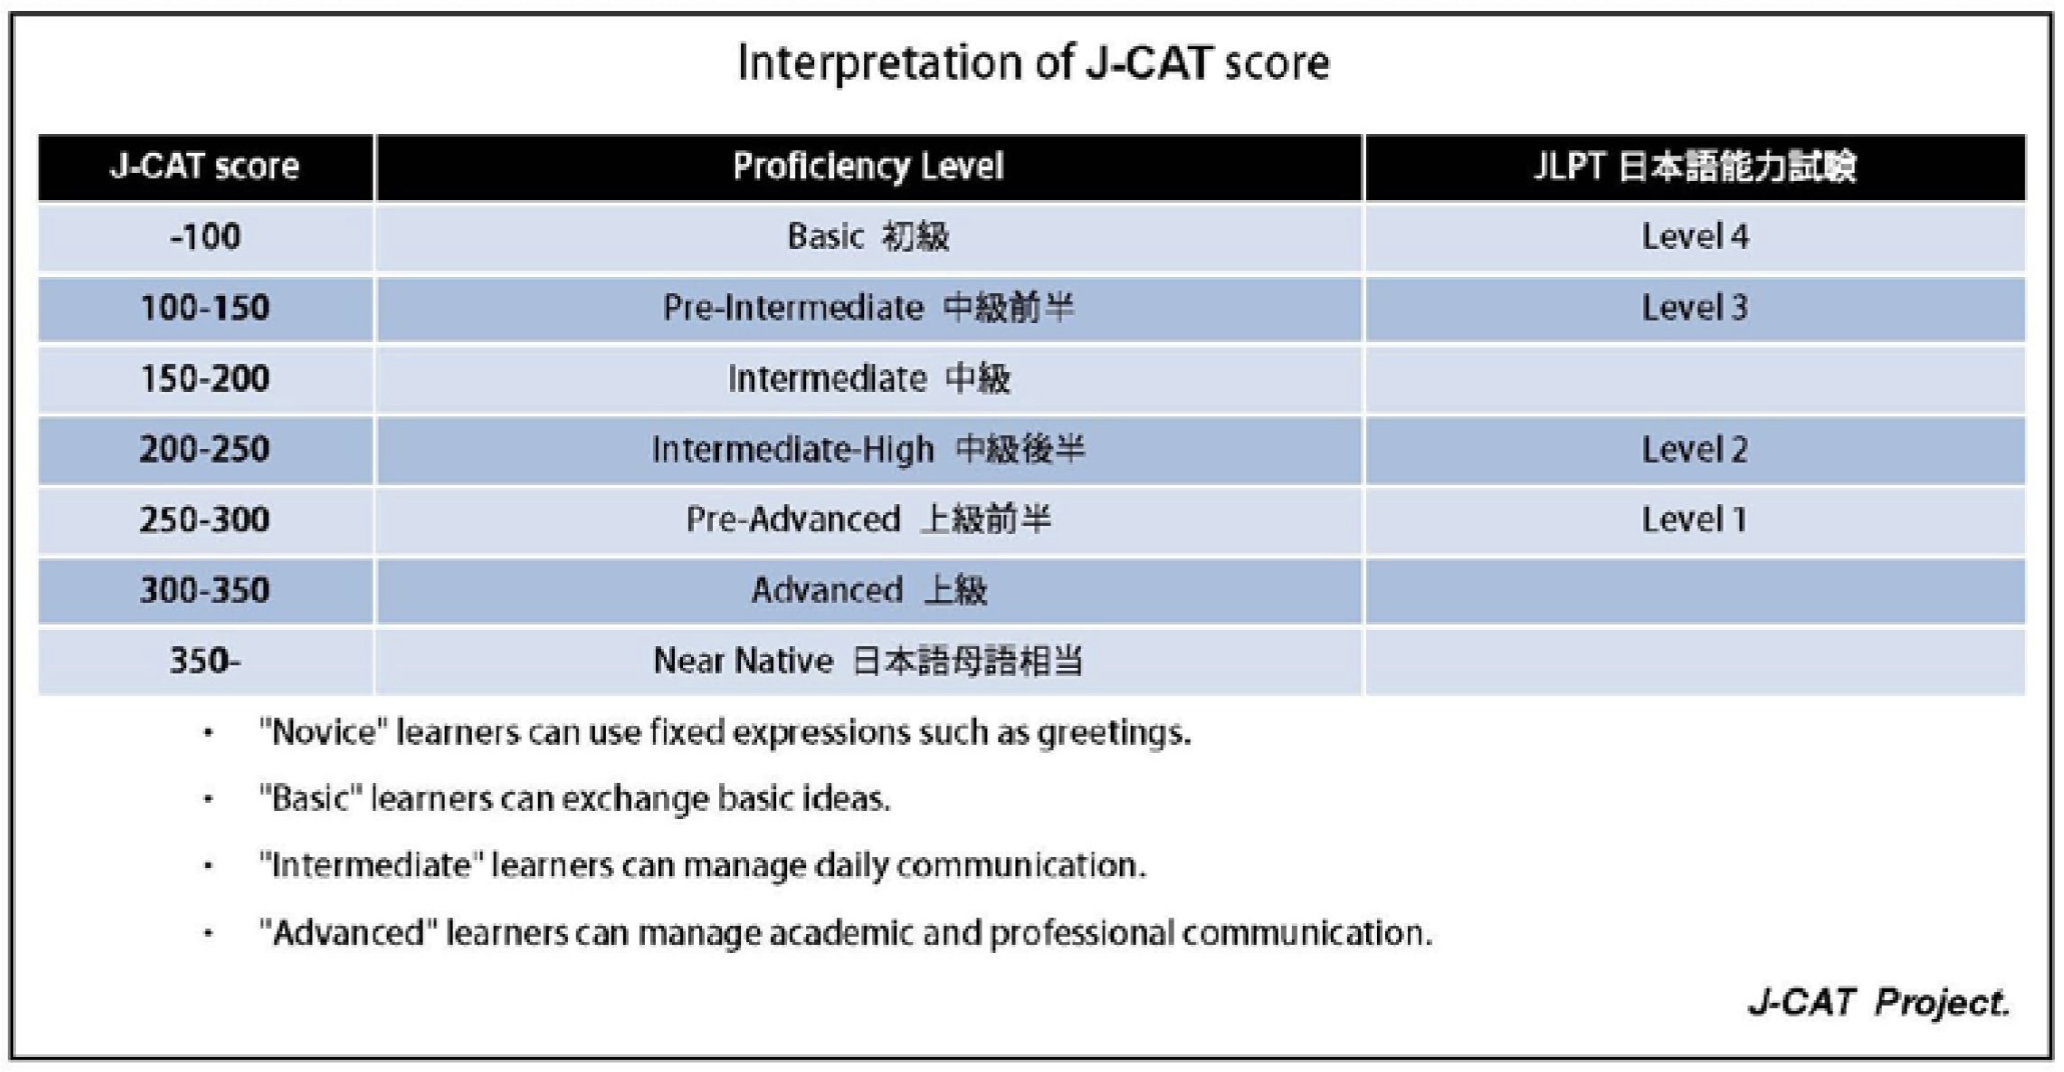
\includegraphics[scale=.3]{img/JCatScores.png}
    \caption[J-Cat Proficency Levels]{The assigned proficency levels from the J-Cat test as taken from the original paper in  2009. Please note that the given JLPT levels do not correspond to the current JLPT test which was reformed in 2010. A new score interpretation connecting JLPT levels to J-Cat scores was released in 2011 and is shown in Table \ref{tab:proficency-table} }
    \label{fig:JCatLevels}
\end{figure}

Each student receives a numerical score that corresponds to one of seven distinct proficiency levels, as detailed in
Table \ref{tab:proficency-table}. This study will categorize participants according to their J-Cat proficiency level. Participants in the
native speaker control group were given a default J-cat score of 999.

\begin{table}
\centering
\begin{tabular}{lrl}
\hline \textbf{JLPT Proficiency Level} & \textbf{J-Cat Score}  \\ \hline
N5 & 0 - 149 \\
N4 & 150 - 199 \\
N3 & 200 - 249 \\
N2 & 250 - 299 \\
N1 Pre-Advanced & 300 + \\
\hline
\end{tabular}
\caption[Proficency Levels]{Proficency level classification based on J-cat score taken from \cite{jcat_interpretation_guide}.}
\label{tab:proficency-table}
\end{table}

\subsection{Writing Tasks}

% add the additional SW 1 and 2 tasks where participants were expected to write a story based on a picture.
Each participant submitted four samples of writing for specific tasks:
\begin{itemize}
    \item A short essay titled "Our Eating Habits," involving a comparison between fast food and home-cooked meals in the learner's home country.
    \item A letter addressed to a former teacher, requesting a letter of recommendation for a scholarship application.
    \item An email seeking an extension for the deadline of a report submission.
    \item An apology email in which the learner must decline an invitation.
\end{itemize}
These tasks were consistent across all participants, regardless of their proficiency levels, and encompassed various task types. The inclusion of a range of task types and formalities was intended to encourage diverse responses from the students and mitigate a potential "task effect" similar to what  was described in \cite{Alexpoulou2017}. The writing samples were processed-as-is without being corrected for learner errors.

\section{Complexity Measures}
detail the complexity measures I will use, how I developed the scripts to automatically "extract them" and the statistical significance between the proficiency levels
list, Sent Length, Clauses per sentence, Noun phrase length,  Subordination, coordination, noun phrase length, MTLD,Morphological complexity? , ADD measures?

lexical sophistication measures use this corpus: \cite{BCCWJ_List} and article citation: \cite{maekawa2014}, Think
about the Tsukuba web corpus also...
When implementing LFP punctuation is removed from the text. Need to mention how text is tokenized in japanese: in
the freq list ばいい is written but would be tokenized as ば and いい ...how to overcome this? Remove verbs? should I use
tokenizer to split the verbs in the word list??

mention the difficulties in finding clauses - specifically in discriminating between coordinate and subordinate
automatically.  POS label SCONJ for subordinate conjunction is used even in the case of coordination, therefore
other methods are needed.

\section{Criterial Features}
Describe the rule based feature matcher I made for extracting certain grammar patterns to disconcern their use
across proficiency levels. Mention how many grammar points at each level I was able to include. Use of the lower
levels doesn't disconcern much so focus should be on the intermediate and upper levels.  Forms that are mainly form
based(and therefore easier to pattern match) should be given priority over. Give some examples of rules derrived

mention that I chose forms which spanned multiple levels. I.e. しか at N4 used with Nouns and しか〜ないat N3 used
with verbs to see if their use at the different levels actually follows this.

don't forget about implementing normalization.

\section{EBMS}
 Here I will give a brief overview of Explainable boosting machines and why I chose them for my analysis.


 % Methodology

\chapter{Evaluation} 
This chapter presents an evaluation of the initial results from the collected data focusing on statistics relating to
developmental trajectories in order to identify potential developmental indices. These findings serve as the
foundation
for the feature selection used in training the explainable boosting machine. Features that demonstrate strong
performance here may also be identified as important by the EBM. The following questions will be addressed in this
section:

\begin{enumerate}
    \item Which measures show an overall developmental trajectory across JLPT levels?
    \item Which features significantly discriminate between proficiency levels, and is a developmental trajectory
    apparent across these levels?
\end{enumerate}

\section{Complexity Measures}

Many of the complexity measures demonstrated trends that correspond to increasing proficiency. However, the patterns
varied across measures. Some showed a consistent increase,while others
decreased, or plateaued at the
higher levels. Notably, most measures were unable to distinguish between the N1 and native speaker (NS) groups.

Statistical analyses were conducted using ANOVA to test for significance, followed by Tukey's HSD test to identify
significant pairwise differences between adjacent proficency levels.

\subsection{Syntactic Complexity Measures}

%Sentence Length
    %discriminates between ajacent proficency levels.
%Clause per Sent
    %*Statistically significant difference between all adjacent levels except N1 and NS

Many of syntactic measures failed to show significant differences between N1 and NS groups. This however is not
cause for concern as the Native speaker group is not actually part of the JLPT scale and is used as a benchmark to
compare how close to native like speech the other learner's are. Therefore when it is mentioned that a measure
distinguished all adjacent levels this means all levels within the JLPT proficency scale not including the native
speaker group.
However several measures
such as sentence length, clauses per sentence, and coordinating clauses per sentence exhibited statistical significance
across most
adjacent proficency levels. These patterns are illustrated in Figures \ref{fig:sentLen}, \ref{fig:cpersent}, and
_____ respectively.

\begin{figure}[htbp]
    \centering
    \begin{minipage}{.48\textwidth}
        \centering
    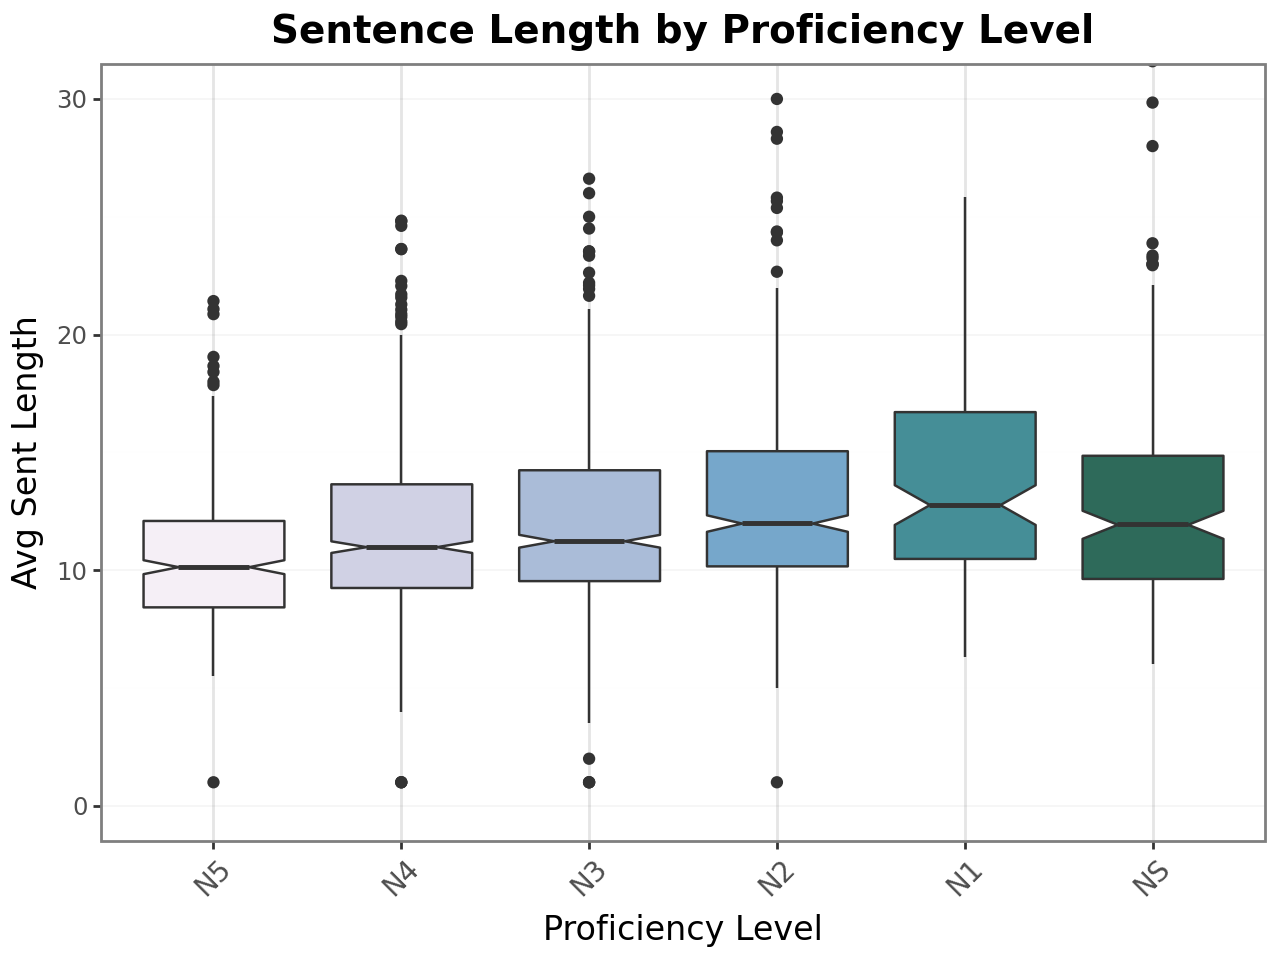
\includegraphics[scale=.3]{img/sentence_len}
    \caption[Average Sentence Length across JLPT levels]{Average Sentence Length across JLPT levels}
        \label{fig:sentLen}
    \end{minipage}
    \hfill
\begin{minipage}{.48\textwidth}
        \centering
        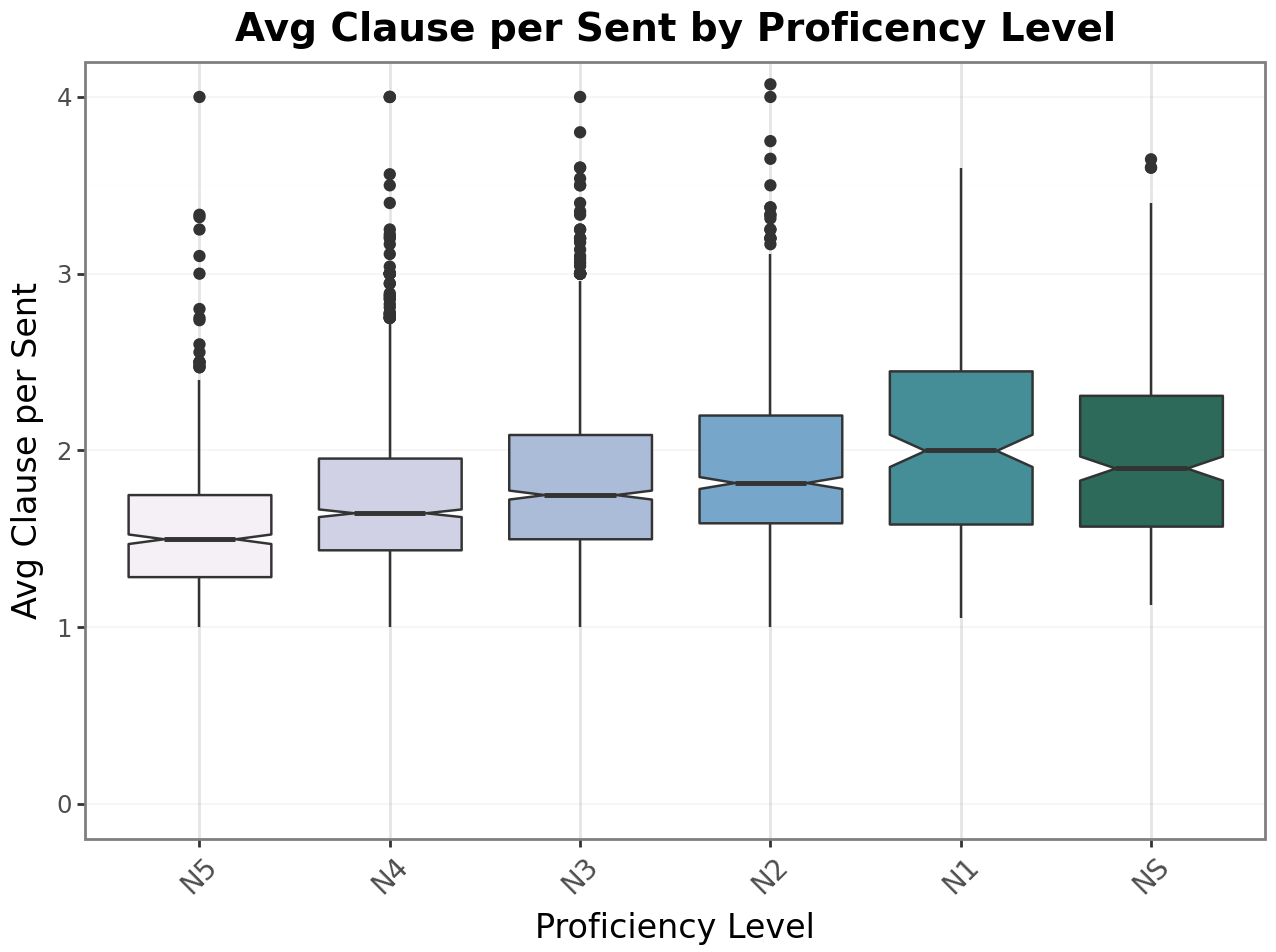
\includegraphics[scale=.3]{img/clausesSent}
        \caption[the ratio of clauses per sentence]{Plot showing the ratio of clauses per sentence}
\label{fig:cpersent}
\end{minipage}
    \end{figure}


\subsubsection{Length-Based Measures}

Length-based metrics capture the amount of syntactic material produced per unit (e.g. per sentence, per clause,
etc.) and are surface level-indications of syntactic complexity. Sentence length exhibited a general upward trend
across proficiency levels and was statistically significant at distinguishing across most adjacent levels, although
it failed to distinguish N1 from the NS group. This aligns
with
the idea that more advanced learners integrate more elements into a single sentence.

Noun phrase length and verb phrase length in contrast, were less informative. NP length remained relatively stable
and did not significantly differ across levels. Verb phrase length did show a weak upward trend but lacked
statistical significance to distinguish between the proficiency levels.

\subsubsection{Clause-Based Measures (Including Coordination/Subordination)}
Clause based measures focus on how learners structure and link clauses, capturing syntactic elaboration through
subordination and coordination.
%Clause Length
%    *N1 and N3 statistically significant difference observed
%    *slightly increases across levels.
%    *Could be influenced by tasks?. Try Removing SW1 and SW2 tasks

Clause length showed a slight
increase across proficiency levels, with a statistically significant difference in distinguishing between N1 and N3.
However, when the SW1 and SW2
tasks were removed, this measure distinguished between all adjacent upper proficiency levels, suggesting a at a
possible
task effect. increases in clause length were more pronounced at the advanced stages than at the beginner levels,
hinting at its potential in detecting finer gradiations of advanced proficiency.

%add other citations
Across prior studies on l2 syntactic development, a common finding is a decrease in coordination and an increase in
subordination with proficiency \citep{Vyatkina2012, Lu2010,Lu2011}. However, in the present data, this trend was not
entirely replicated. One reason may be the early introduction of subordinating conjunctions in Japanese L2
instruction such as 「から」(kara, \textit{because}) and 「けど」(kedo, \textit{but}) which are frequently used without
requiring transformation of verbs or deep syntactic embedding.

%Subordinate Clauses per Sent
    %statistically significance difference between N5 and N4 ,and then N1 and N3 but does not discriminate between the
%higher proficency
    %levels. Subordination is taught quite early to L2 speakers, could this be why?
%Subordinate Clause per clause
    %statistically significant difference between N5 and N4 and N4 and N3,
    %slight decrease across levels showing a prefernce for different clause types in the higher levels?

The measure of subordinate clauses per sentence showed a modest increase across proficiency levels and was
statistically significant in distinguishing lower levels(N5 vs N4) and non-adjacent upper levels (N3 vs N1). This
reflects developmental progression but not ina  linear fashion (see Figure~\ref{fig:SubclperS}).

In contrast, the ratio of subordinate clauses to total clauses showed a decreasing trend, with significant
differences observed between non-adjacent levels (N5 vs N3, N4 vs N2).  As shown in Figure~\ref{fig:SCperC}, this
suggests that lerners at higher proficiency levels may diversify their clause structures and shift toward more
coordination or other complex constructions.

\begin{figure}[htbp]
    \centering
    \begin{minipage}{.48\textwidth}
        \centering
    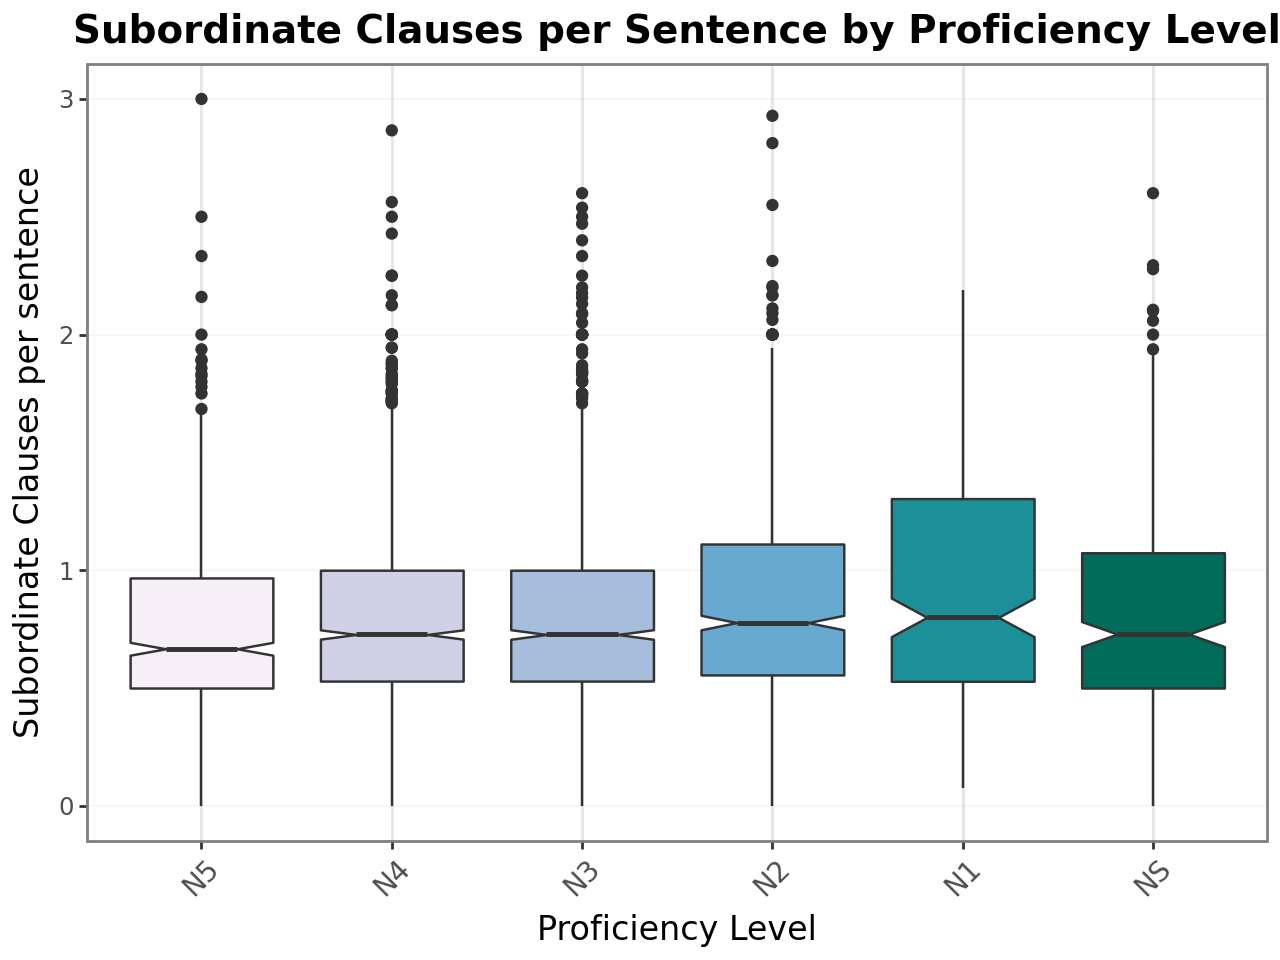
\includegraphics[scale=.3]{img/SCperS}
    \caption[Average subordinate clauses to sentences across JLPT levels]{Average subordinate clauses to sentences across JLPT levels}
        \label{fig:SubclperS}
    \end{minipage}
    \hfill
\begin{minipage}{.48\textwidth}
        \centering
        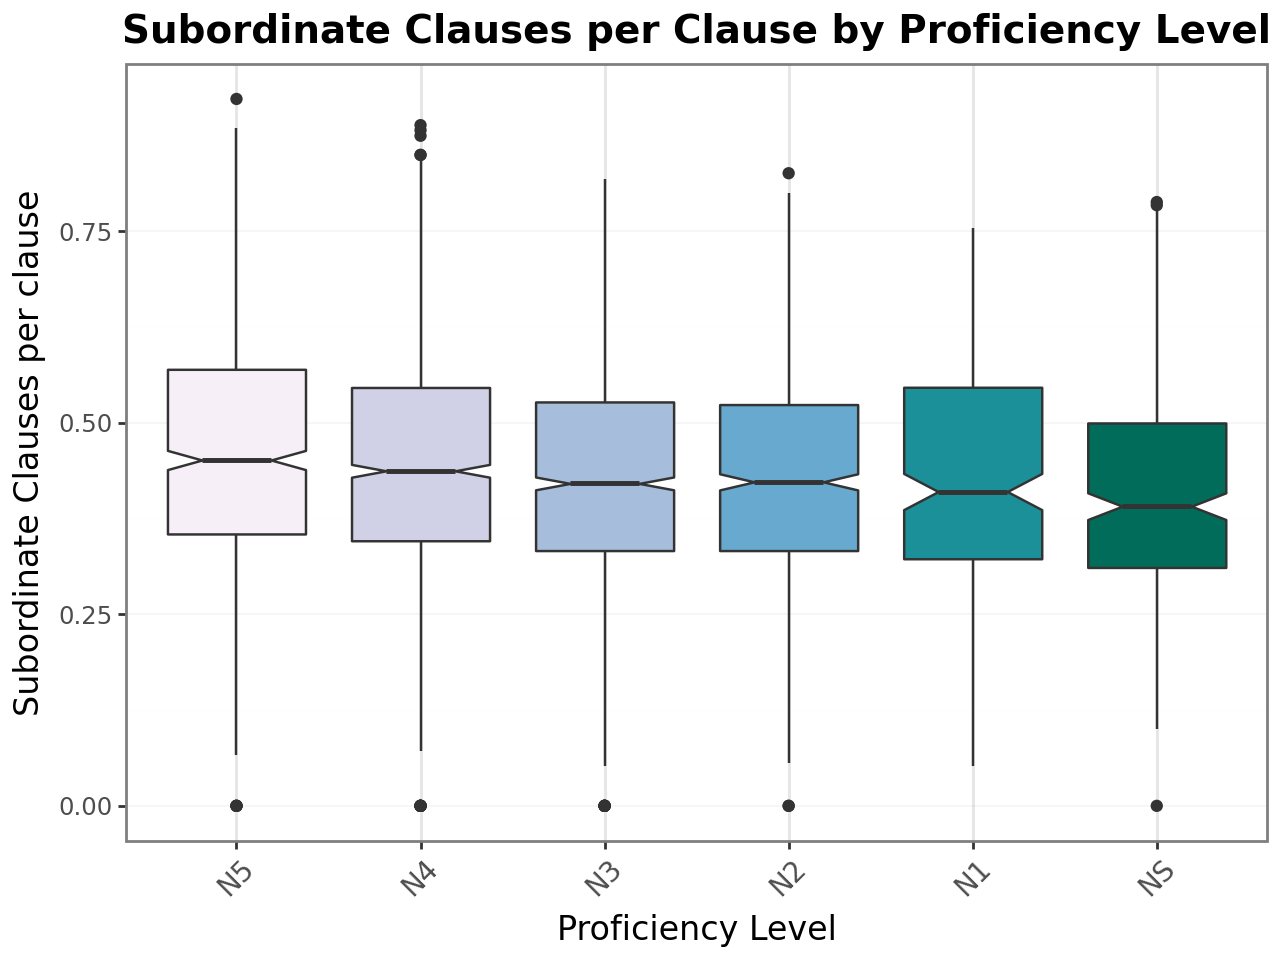
\includegraphics[scale=.3]{img/SCperC}
        \caption[Average subordinate clauses to clauses ratio across JLPT levels]{Average subordinate clauses to clauses ratio across JLPT levels}
\label{fig:SCperC}
\end{minipage}
    \end{figure}

%Coordinating Conjunction per Sentence
    %*Statistically significant in distinguishing all adjacent levels except N1 and NS group
    %*Also increases across prof levels, could be due to the fact that SC are taught first.
%Coordinating Conjunction per Clause
    %*increase across prof. levels
    %*Statistically significant between levels except N2 & N1 and N1 & NS
%Subordinating Clauses to Coordinate Clauses
%    *statistically significant for every other proficency level. ie. N5 & N3, N3 & N1, N2&N4
%    *variance also increases at the higher proficency levels but , maybe due to more CC being used?

Measures related to coordination showed strong developmental patterns. The number of coordinate clauses per sentence
increased across levels and significantly
distinguished all adjacent levels. This trend may reflect increased syntactic range at higher levels where
coordination is used stylistically or rhetorically, not just structurally (Figure~\ref{fig:CCperSent}).

Similarly, coordinate clauses per clause also increased with proficiency and distinguished most adjacent levels
except N2 - N1 (Figure~\ref{fig:CCperCl}). These findings contrast with typical L2 development models by maybe due
to the instructional sequence in Japanese, where simple subordinate forms are taught earlier and coordination
becomes more common as learners diversify their expression.

The ratio of subordinate clauses to
coordinate clauses further supports this shift. It showed statistically significant differnces between non-adjacent
levels (N5 vs N3, N3 vs N1) and increased variance at higher proficiency levels, possibly reflecting more
individualized or task-drive distribution of clause types.

\begin{figure}[htbp]
    \centering
    \begin{minipage}{.48\textwidth}
        \centering
    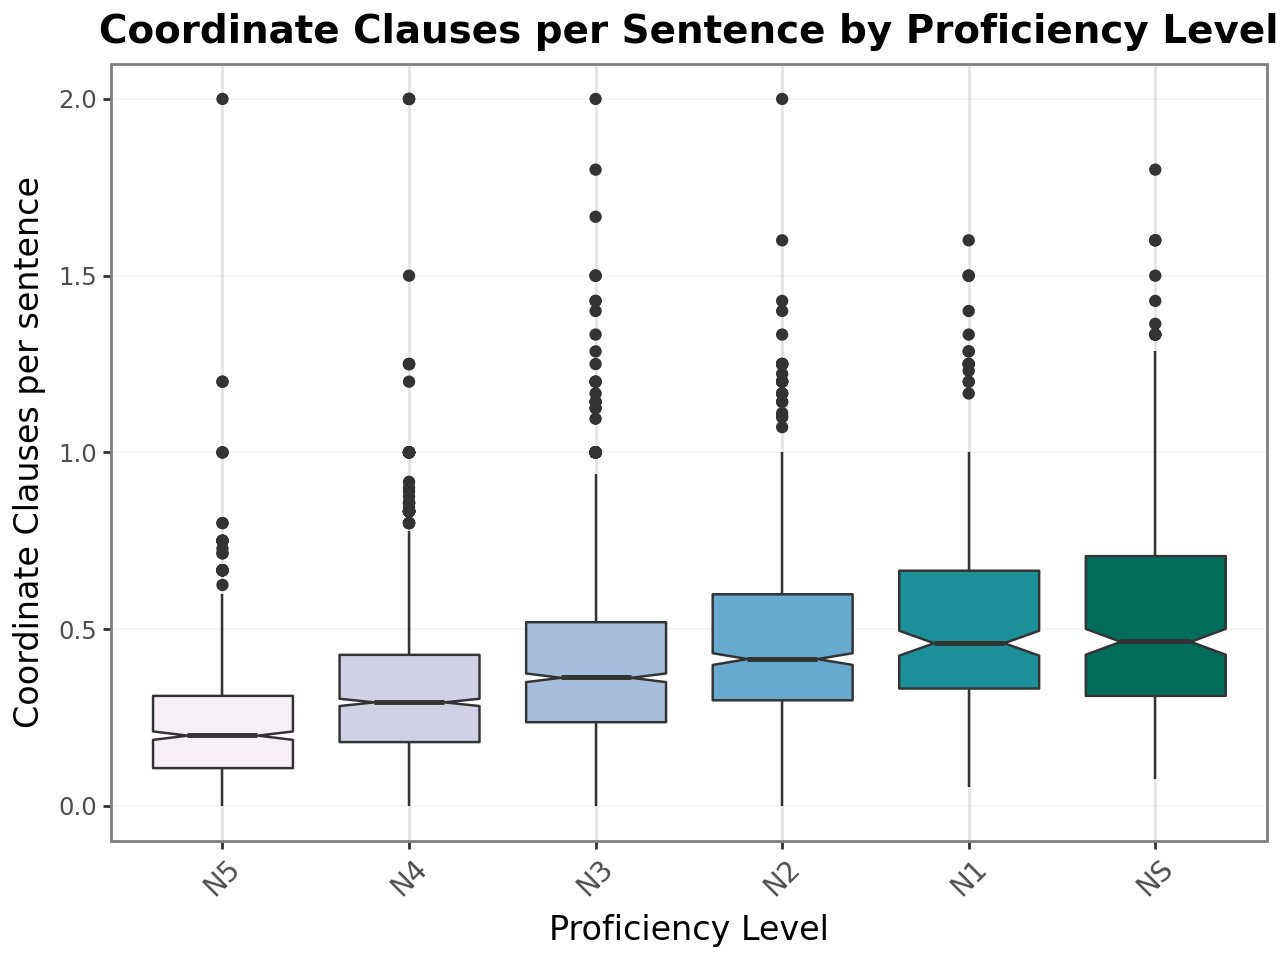
\includegraphics[scale=.3]{img/CCperSent}
    \caption[Average coordinate clauses to sentences across JLPT levels]{Average coordinate clauses to sentences across JLPT levels}
        \label{fig:CCperSent}
    \end{minipage}
    \hfill
\begin{minipage}{.48\textwidth}
        \centering
        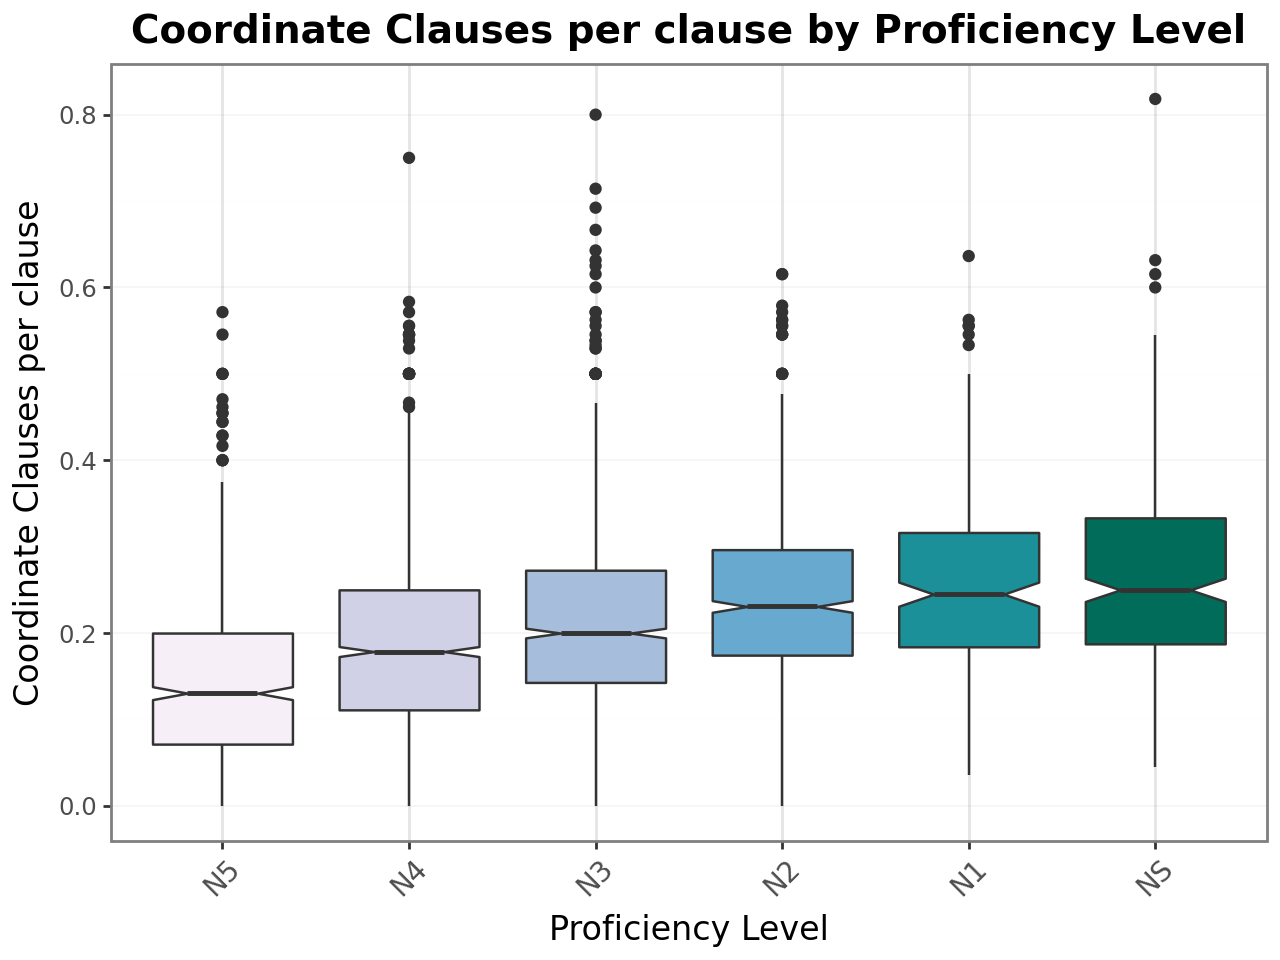
\includegraphics[scale=.3]{img/CCperC}
        \caption[Average coordinate clauses to clauses ratio across JLPT levels]{Average coordinate clauses to clauses ratio across JLPT levels}
\label{fig:CCperCl}
\end{minipage}
    \end{figure}

%CC Freq
    %no significant difference between any of the levels and no clear pattern...
%SC Frequency
    %*increases across levels
    %*Significant between n5&N4, N4&N3, N3&N2, N2 & NS
Normalized frequencies of subordinating and coordinating conjuctions were analyzed as a proxy measure as done in \citet{Vyatkina2012}, however, they showed mixed results. Subordinating conjunction frequecy increased across proficiency levels and showed statistically significant differences at lower levels (N5 vs. N4, N4 vs N3), reflecting early acquisition and frequent use. Coordinating conjunction frequency, however, did not show significant variation across levels and did not follow a clear developmental trend. This may be due to extraction limitations or the realtively sparse distribution of explicit coordinators in learner texts.

\subsubsection{Dependency-Based Measures}

Dependency-based measures provide a structural perspective on syntactic complexity by quantifying how syntactic
units are hierarchically and linearly related. Unlike length or clause-based measures, which capture surface level
elaboration, these metrics reflect the cognitive load and integration required to process or produce a sentence.
Both measures considered, Mean Dependency Distance (MDD) and Mean Hierarchical Distance (MHD), showed strong
associations with increasing proficiency and can be considered promising indicators of developmental progression.

%MDD
    %* Statistically significant between every other level as well as the higher proficency levels N3&N2 and N2&N1
    %*no significant between N1 and NS
    %*Increase across levels
As shown in Figure~\ref{fig:mdd}, MDD increased consistently across proficiency levels and was statistically
significant between most levels, including higher-level distinctions such as N3 vs. N2 and N2 vs. N1. The consistent
upward trajectory suggests that as learners become more proficient, they are able to manage longer dependency
relations, producing more integrated syntactic structures.

%MHD
%    *Increase across levels
%    *statistically significant between all adjacent levels except NS and N1

Similarly, MHD, depicted in Figure~\ref{fig:mhd}, also exhibited a steady increase with proficiency. It was
statistically significant across all adjacent levels. This measure captures the hierarchical depth of sentence
structure, and its strong performance across levels supports the idea that syntactic embedding becomes more complex
and frequent as learners advance.

\begin{figure}[htbp]
    \centering
    \begin{minipage}{.48\textwidth}
        \centering
    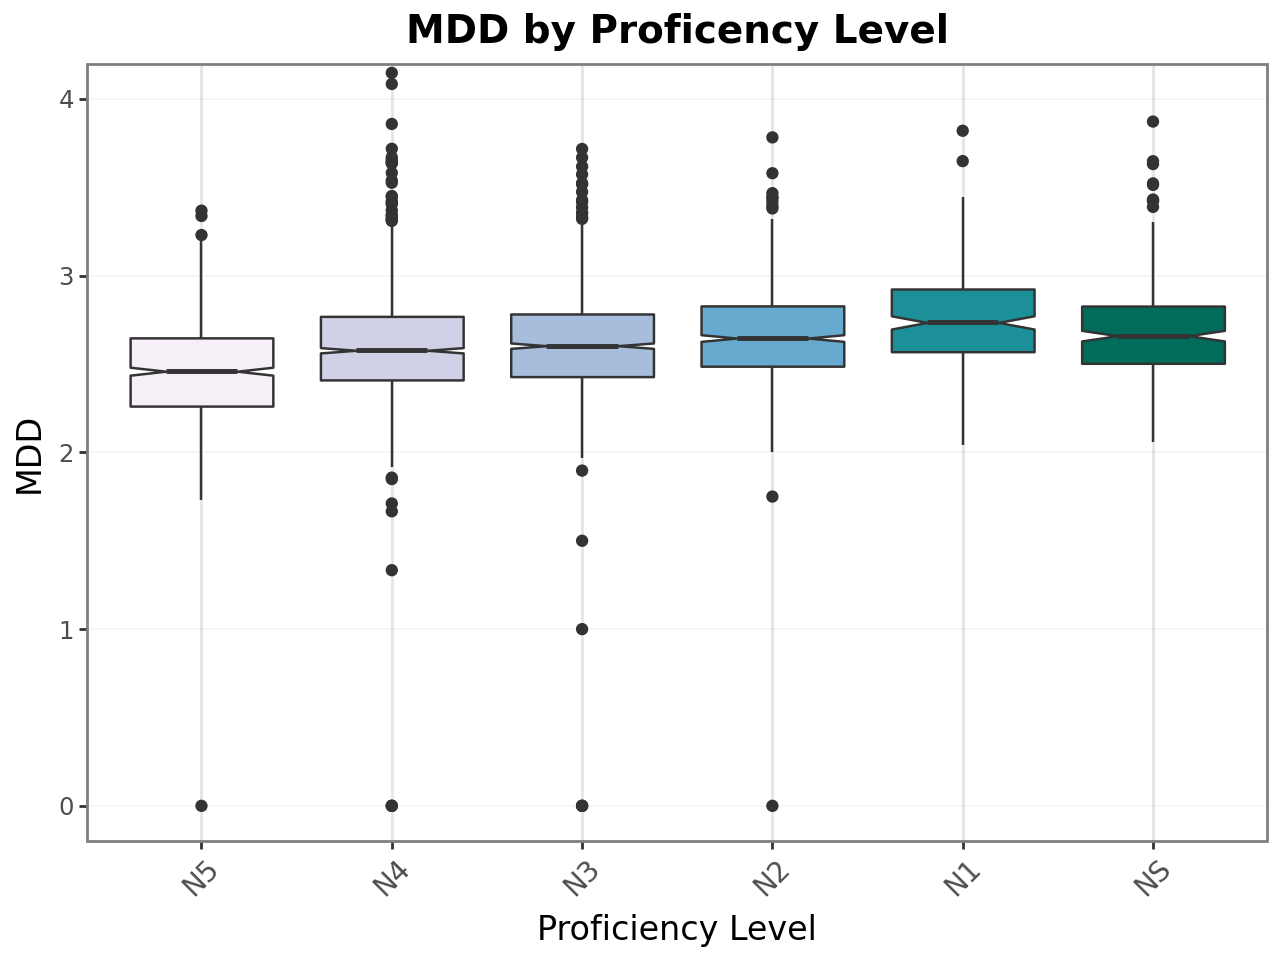
\includegraphics[scale=.4]{img/MDD}
    \caption[Mean Dependency Distance across JLPT Proficency Levels]{Mean Dependency Distance (MDD) increases steadily across JLPT levels, with significant differences between most levels.}
        \label{fig:mdd}
    \end{minipage}
    \hfill
\begin{minipage}{.48\textwidth}
        \centering
        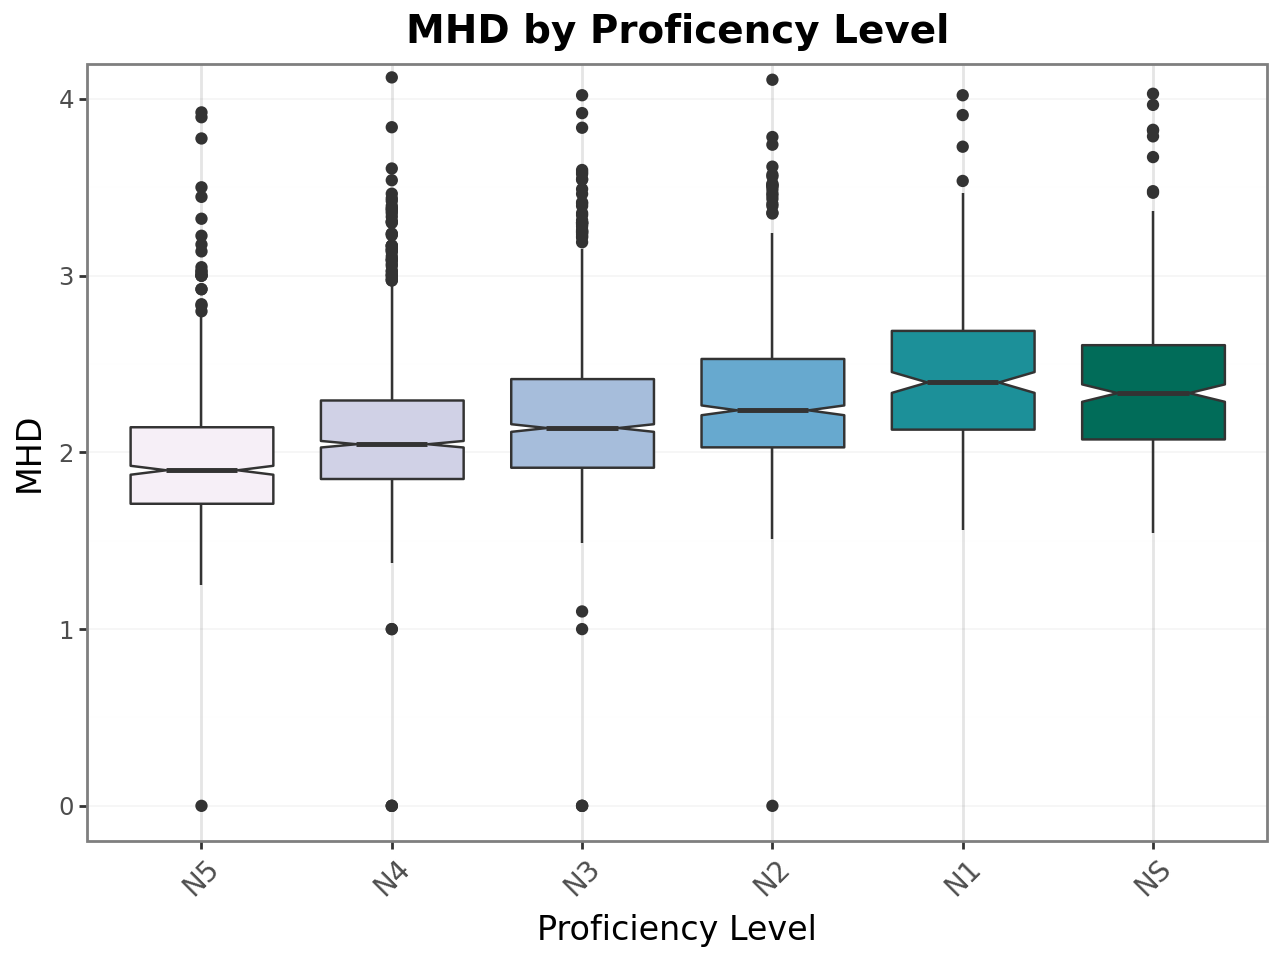
\includegraphics[scale=.4]{img/MHD}
        \caption[Mean Hierarchtical Distance across JLPT Proficency Levels]{Mean Hierarchtical Distance (MHD) increases consistently, distinguishing all adjacent proficency levels.}
\label{fig:mhd}
\end{minipage}
    \end{figure}


\subsection{Lexical Complexity Measures}
Lexical complexity captures the diversity, sophistication and density of vocabulary used by learners. The measures
included to evaluate how vocabulary use changes across proficiency levels include type-based diversity metrics, part
-of-speech (POS) density ratios, and lexical frequency profiles.

\subsubsection{Lexical Diversity Measures}
%CTTR
%    *Discriminates between adjacent levels at the lower proficiency levels,but no statistical significant difference
%    found between N2 & N1 and N1 & NS, and N2 and NS
%    *Generally increases between levels

The Corrected Type-Token Ratio (CTTR) showed a general increase across proficiency levels but was most effective at
distinguishing between adjacent levels in the lower proficiency range (Figure~\ref{fig:cttr}). No statistically significant
differences were
found between N2 vs. N1. This suggests that CTTR may plateau at advanced levels and is more sensitive to early
vocabulary expansion.

\begin{figure}[h]
    \centering
    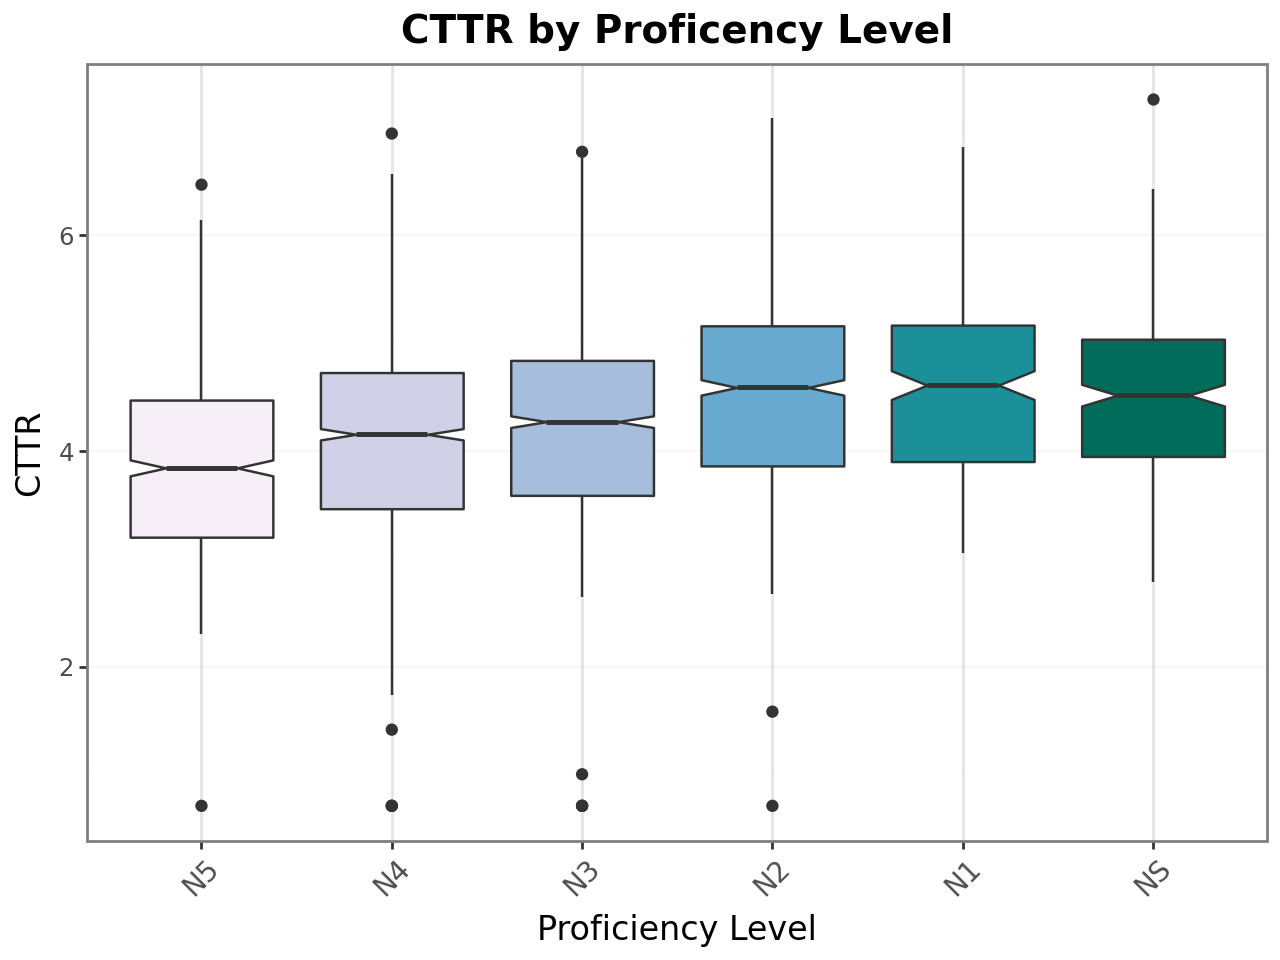
\includegraphics[scale=.5]{img/CTTR}
    \caption[Correct-Type]{CTTR}
    \label{fig:cttr}
\end{figure}

%MTLD-Surface
    %* increases across levels
    %* Statistically significant in distinguishing between lower prof levels.('N2', 'N3'), ('N2', 'N4'), ('N3', 'N5')
%, ('N4','N5')
%MTLD-Inflection
    %*increases across levels not as much as with surface forms
    %* Statistically significant in distinguishing between lower prof levels.('N2', 'N3'), ('N2', 'N4'), ('N3', 'N5')
%, ('N4','N5')

The Measure of Textual Lexical Diversity was calculated for surface forms and lemmas (non-inflected forms). The
MTLD-surface measure increased steadily across proficiency levels and showed statistically significant differences
for several adjacent pairs in the lower and mid-proficiency ranges (N5 vs. N4, N3 vs. N2). This suggest a gradual
increase in word variety as learners develop their langauge (Figure~\ref{fig:mtldS}). The MTLD-lemma measure also
showed an increasing trend, although the effect size was smaller than for surface forms(Figure~\ref{fig:mtldL}). Statistically
significant
differences were observed between similar level pairs, suggesting that while learners increase their morphological
variation, this dimension of diversity develops more slowly.


\begin{figure}[htbp]
    \centering
    \begin{minipage}{.48\textwidth}
        \centering
    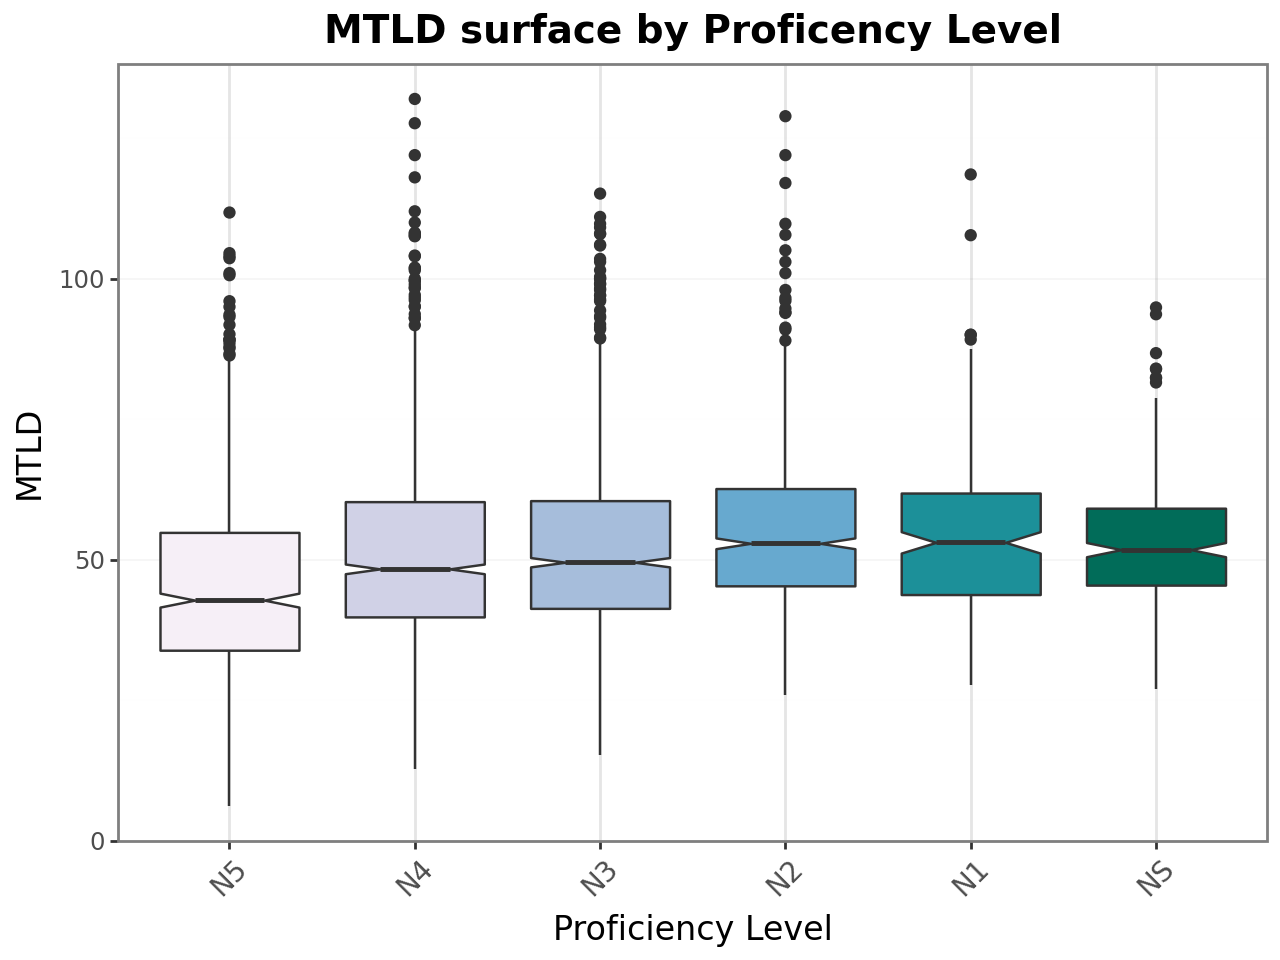
\includegraphics[scale=.4]{img/MTLDsurface}
    \caption[MTLD Surface]{MTLD Surface}
        \label{fig:mtldS}
    \end{minipage}
    \hfill
\begin{minipage}{.48\textwidth}
        \centering
        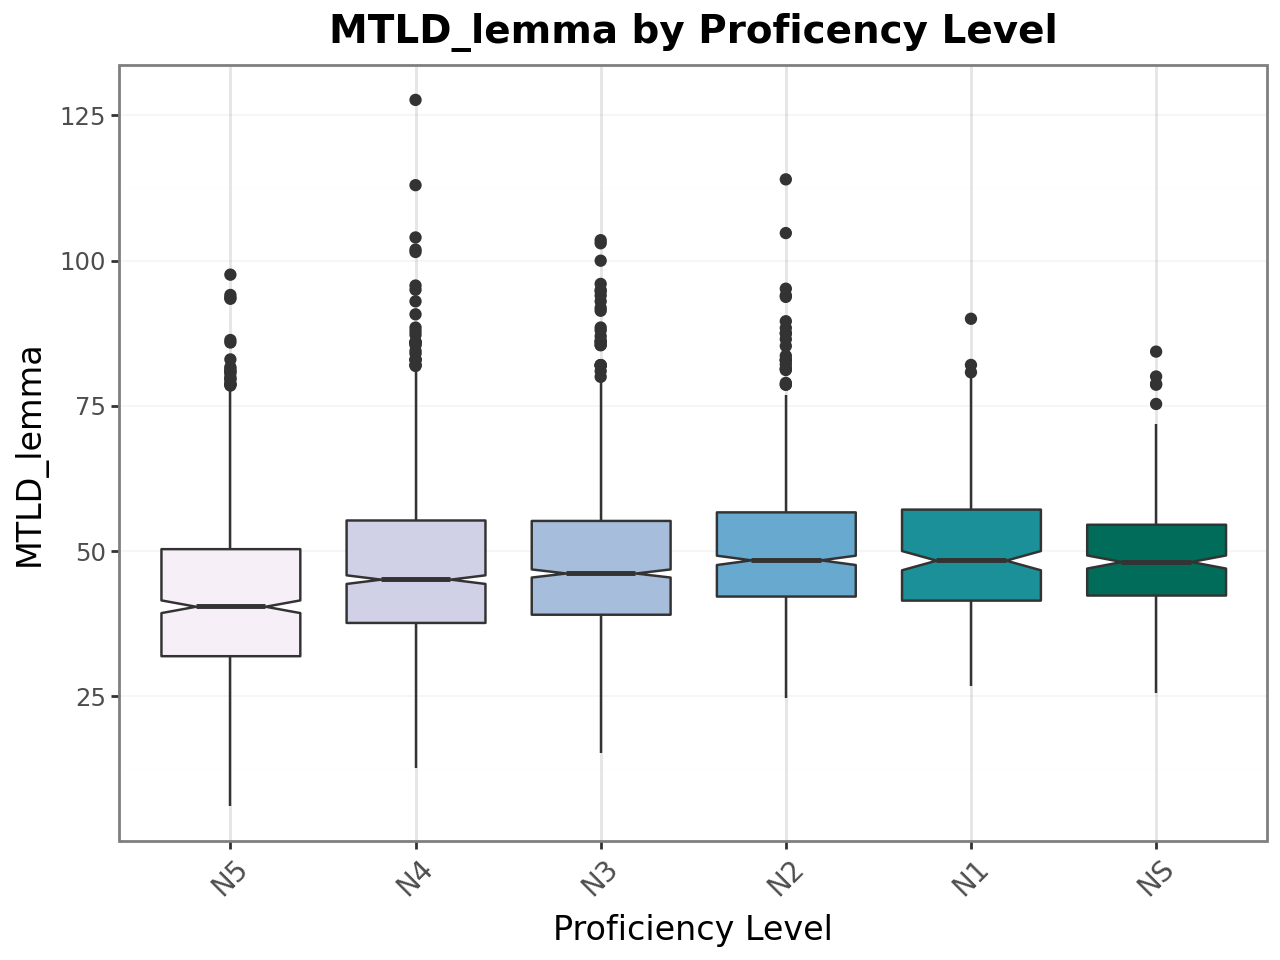
\includegraphics[scale=.4]{img/MTLDlemma}
        \caption[MTLD lemma]{MTLD Lemma}
\label{fig:mtldL}
\end{minipage}
    \end{figure}

\subsubsection{Lexical Density Measures}

Part-of-speech density ratios provide insight into how learners balance content and function words in their writing.
These ratios were normalized by total token count
%Noun Density
    %*Decreases across proficiency levels (null subjects?)
    %*distinguishes beteween lower prof levels. N4 & N5 and N3 and N4 (almost significant p = .06)
%Verb Density
    %*increase across levels
    %* Only statistically significant at distinguishing between lower levels N5 & N4 and N4&N3
Noun density decreased across proficiency levels. This may partially be explained by the use of null subjects in
Japanese, leading to fewer overt noun phrases in more advanced writing (Figure~\ref{fig:nounDen}). Statistically significant
differences were
observed between N5-N4 and N4-N3.

Verb density increased with proficiency but plateaued at the more advanced levels (Figure~\ref{fig:verbDen}) and was only
statistically
significant in distinguishing between the lower adjacent levels (N5-N4 and N4-N3). This pattern suggents that while
verb use expands early, it stabilizes in the upper ranges.

\begin{figure}[htbp]
    \centering
    \begin{minipage}{.48\textwidth}
        \centering
    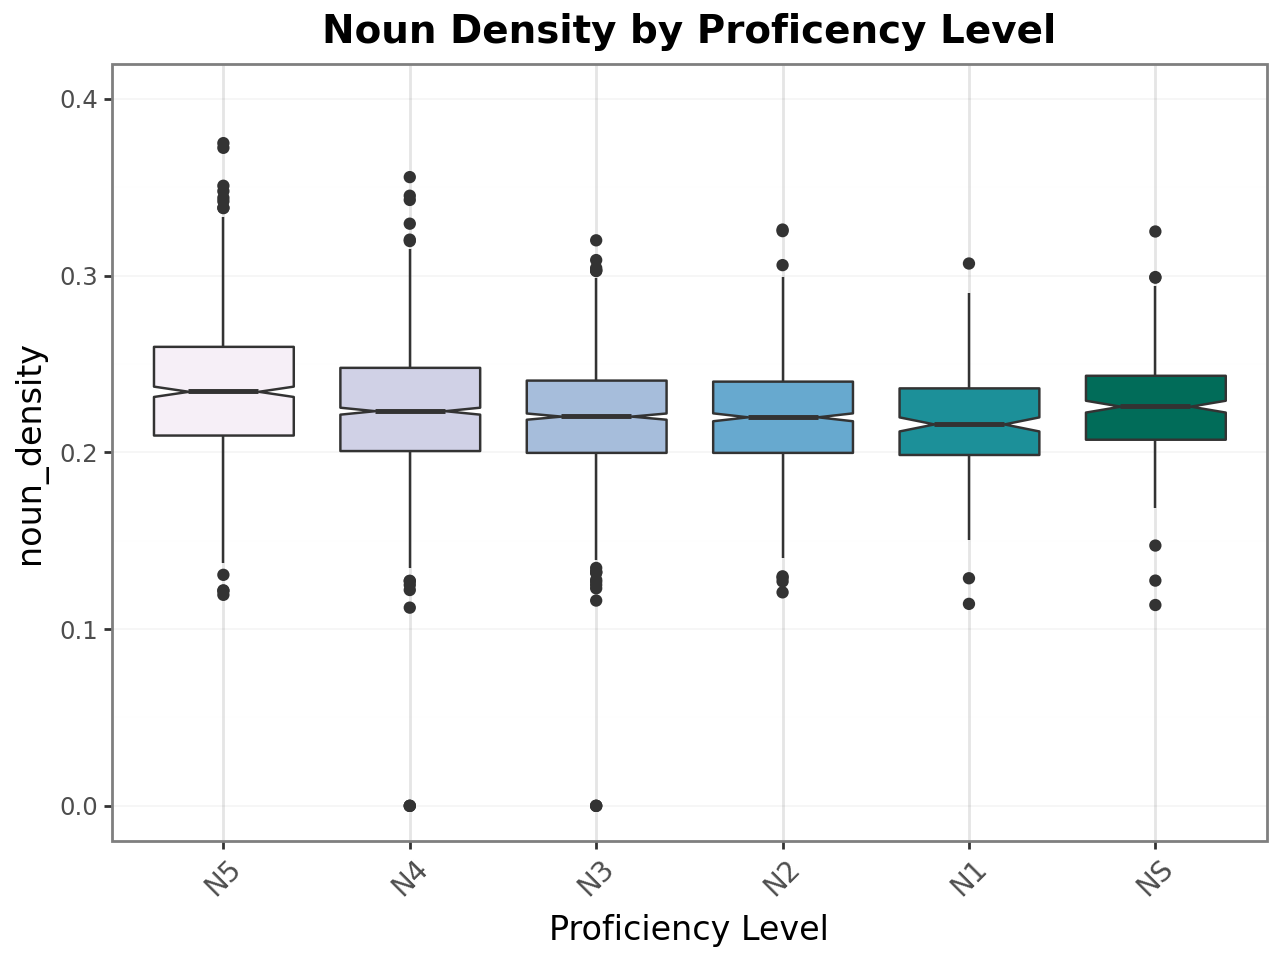
\includegraphics[scale=.4]{img/NounDen}
    \caption[Noun Density Across JLPT Proficiency Levels]{Noun Density}
        \label{fig:nounDen}
    \end{minipage}
    \hfill
\begin{minipage}{.48\textwidth}
        \centering
        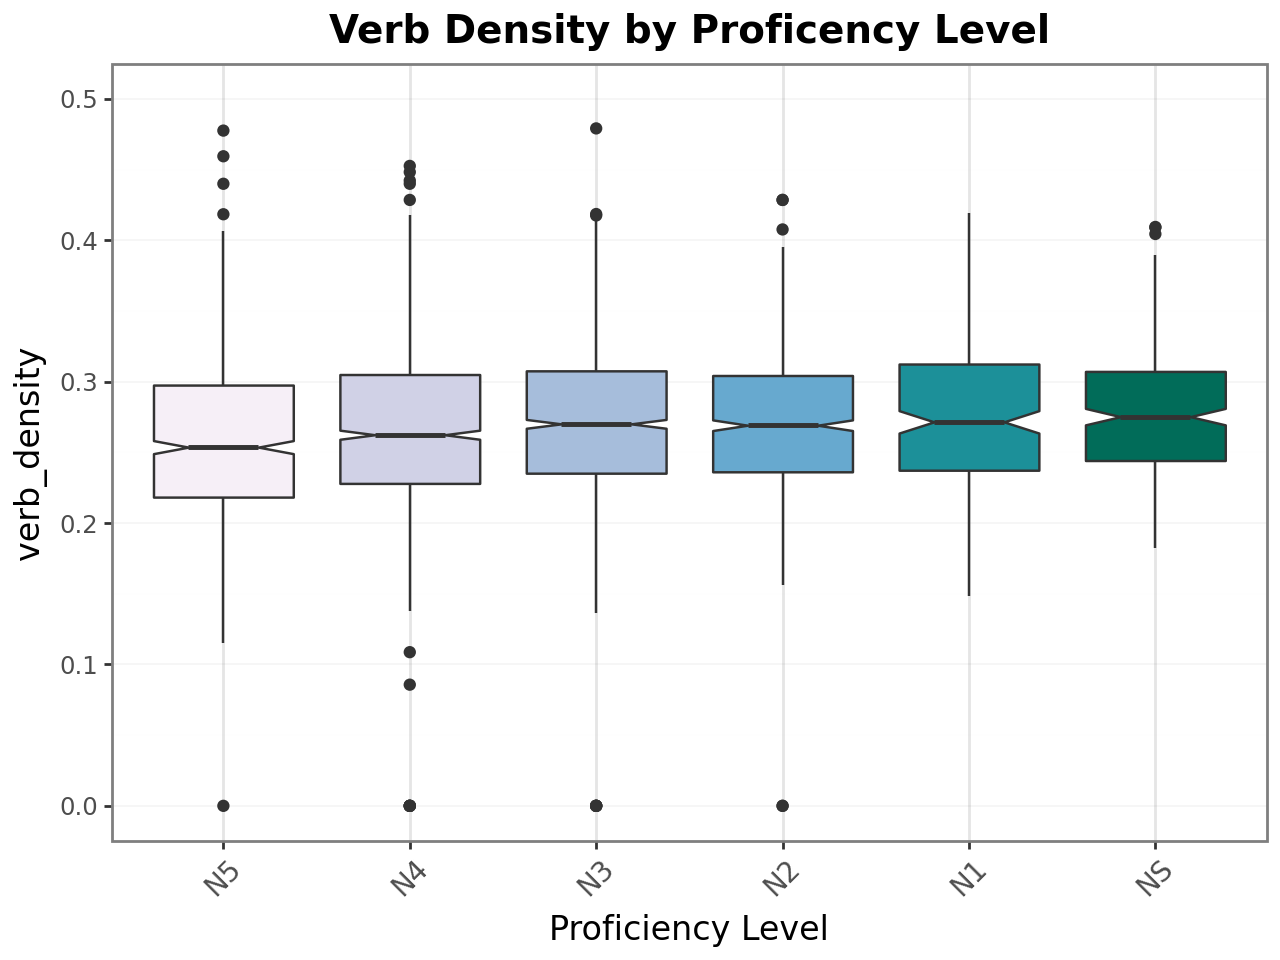
\includegraphics[scale=.4]{img/VerbDen}
        \caption[Verb Density Across JLPT Proficiency Levels]{Verb Density}
\label{fig:verbDen}
\end{minipage}
    \end{figure}


%Adjective Density
    %*Increase across proficiency levels
    %*Statistically significant in distinguishing between lower levels N5&N4, N5&N3, N3&N2
    %*could also be task dependent check later
%Adverb Density
    %*increase across levels except a drop in use for N1 (due to low sample size?)
    %*Statistically significant in distinguishing between lower levels N4&N5, N3&N5 N3&N2
Adjective density showed a consistent increase across proficiency levels and was statistically significant in
distinguishing lower and intermediate pairs (N5-N4, N5-N3, N3-N2). Adverb density also increased across levels, though with a noticeable drop at N1. This may be due to sample size
limitations or task variation. Statistically significant differences were found between N5-N4, N5-N3, and N3-N2,
indicating usefulness in assessment of early-stage proficiency.

\begin{figure}[htbp]
    \centering
    \begin{minipage}{.48\textwidth}
        \centering
    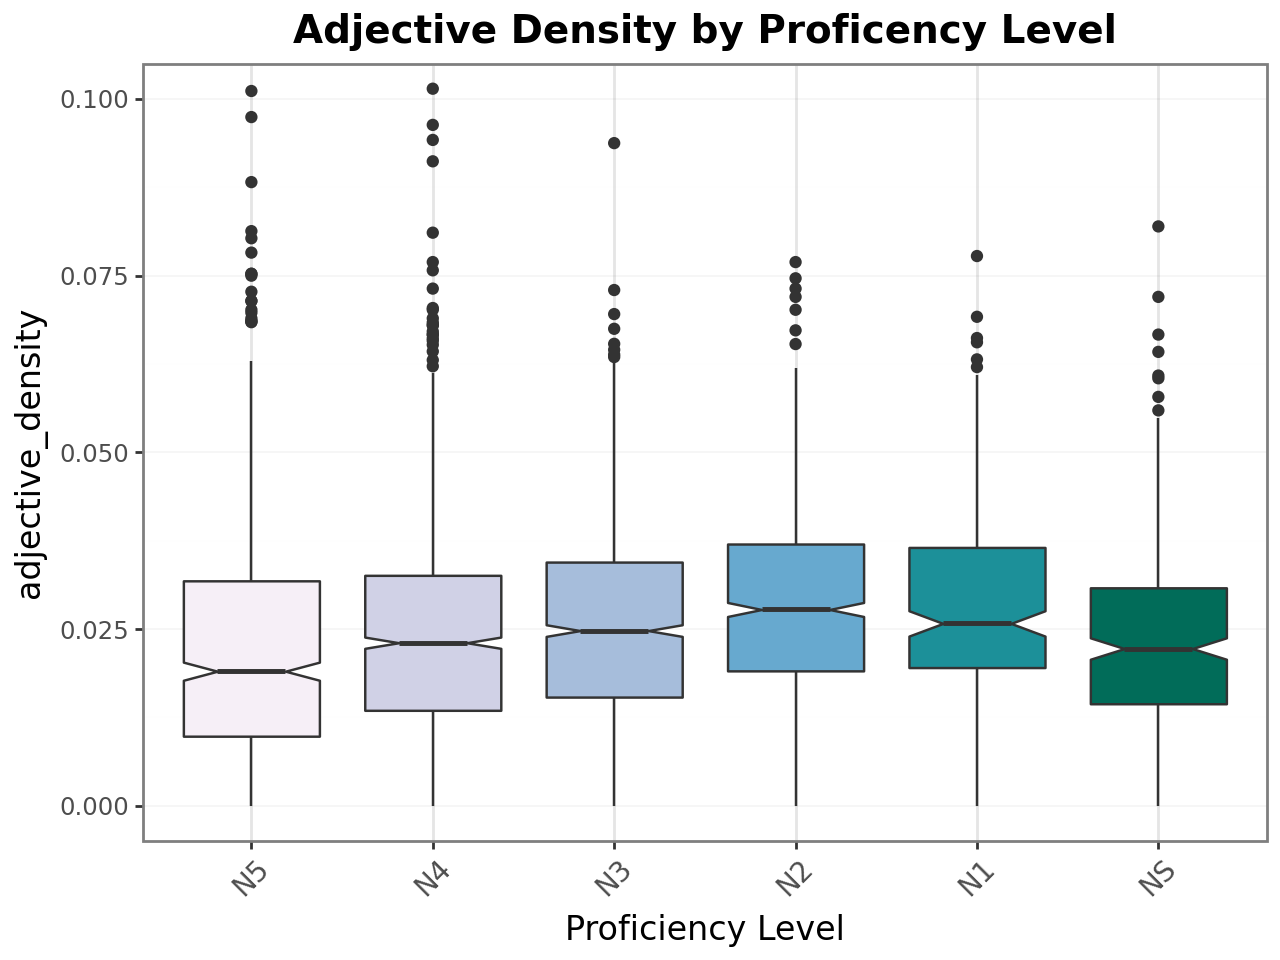
\includegraphics[scale=.4]{img/AdjDen}
    \caption[Adjective Density Across JLPT Proficiency Levels]{Adjective Density}
        \label{fig:adjDen}
    \end{minipage}
    \hfill
\begin{minipage}{.48\textwidth}
        \centering
        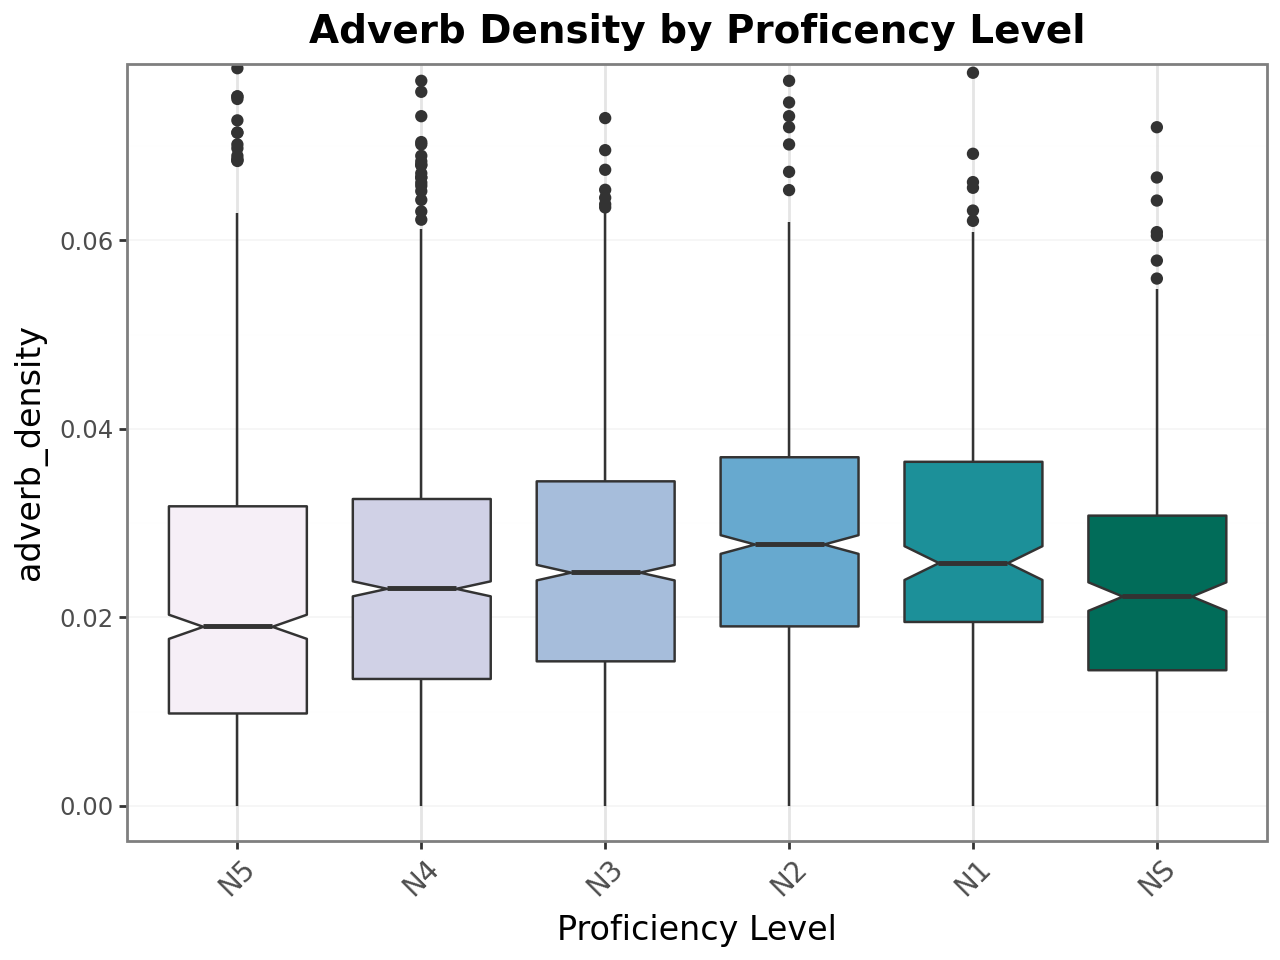
\includegraphics[scale=.4]{img/AdvDen}
        \caption[Adverb Density Across JLPT Proficiency Levels]{Adverb Density}
\label{fig:advDen}
\end{minipage}
    \end{figure}

\subsubsection{Lexical Frequency Profile Measures}
Lexical sophistication was examined using the Lexical Frequency Profile (LFP), and calculated based on two
reference corpora: the
Balanced Corpus of
Contemporary Written Japanese (BCCWJ) \citep{maekawa2014} and a JLPT-aligned wordlist \citep{jisho.org}. These
analyses aimed to capture how learners distribute their vocabulary use across different frequency/proficiency bands
as their proficiency develops.

\begin{figure}[htbp]
    \centering
    \begin{minipage}{.48\textwidth}
        \centering
    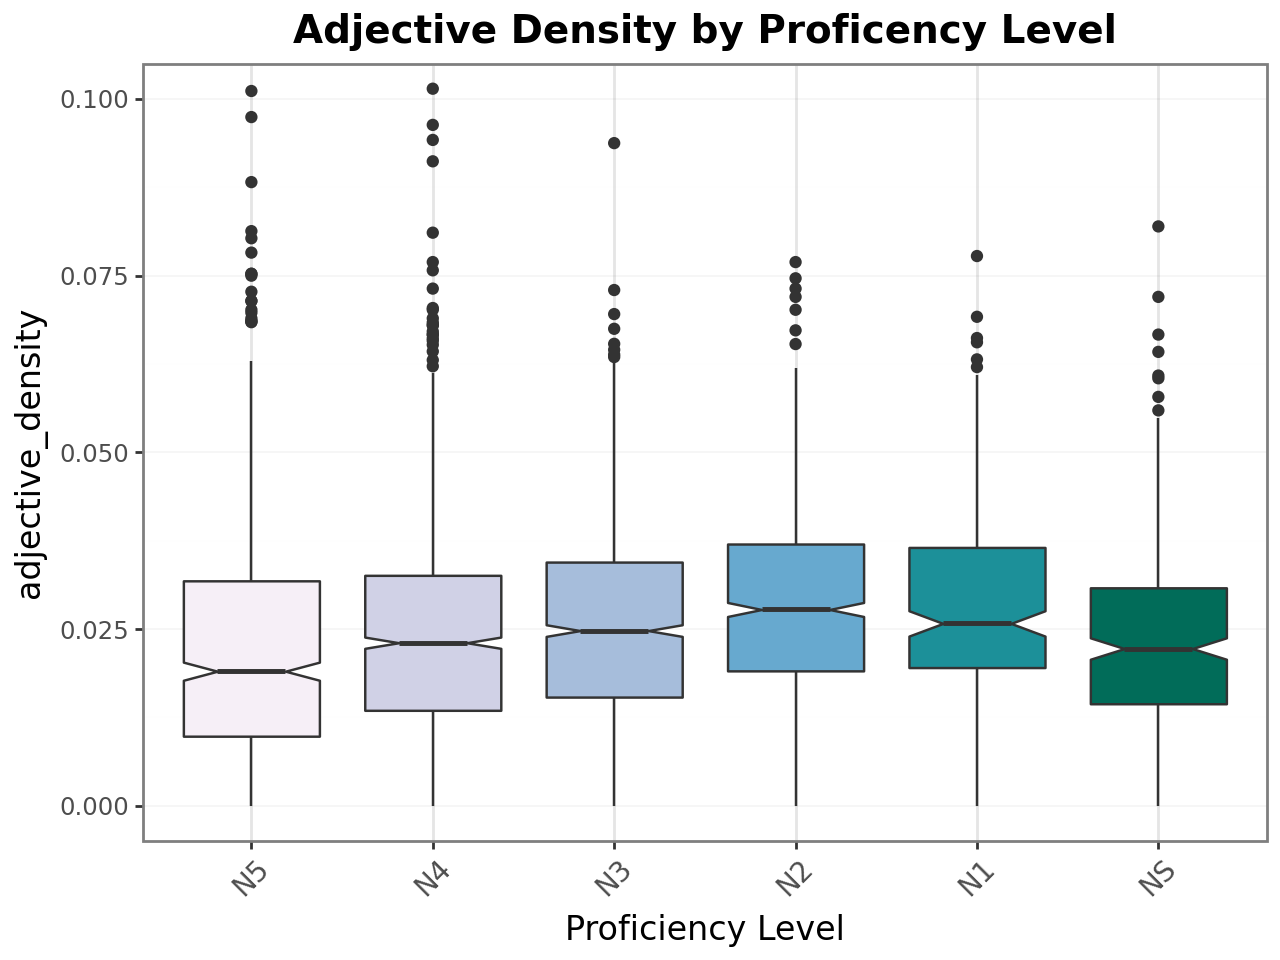
\includegraphics[scale=.4]{img/AdjDen}
    \caption[Adjective Density Across JLPT Proficiency Levels]{Adjective Density}
        \label{fig:adjDen}
    \end{minipage}
    \hfill
\begin{minipage}{.48\textwidth}
        \centering
        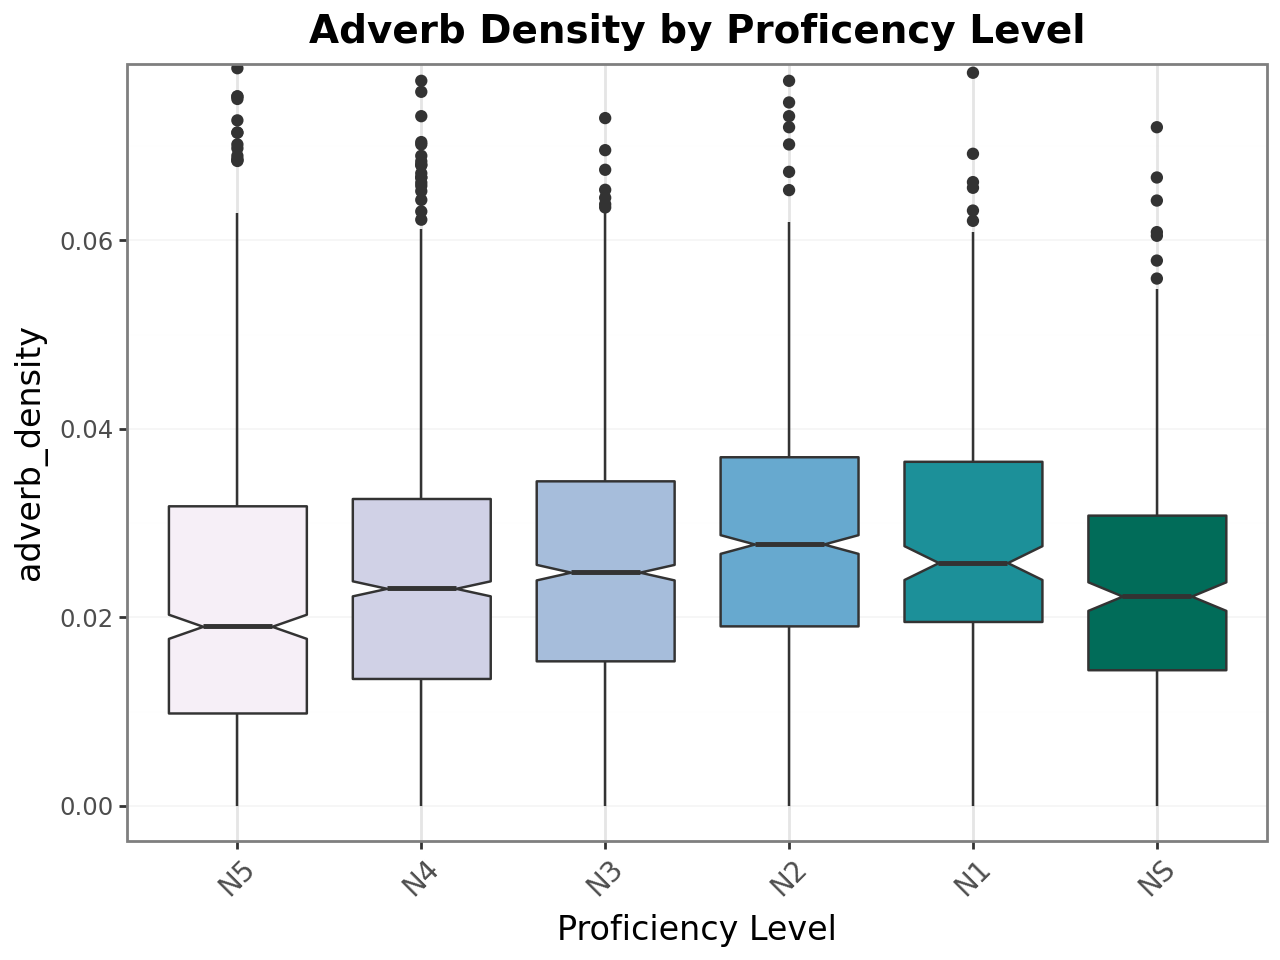
\includegraphics[scale=.4]{img/AdvDen}
        \caption[Adverb Density Across JLPT Proficiency Levels]{Adverb Density}
\label{fig:advDen}
\end{minipage}
    \end{figure}

\subsubsubsection{Balanced Corpus of Contemporary Written Japanese (BWCCJ)}
LFP -BWCCJ Corpus
    * high frequency of items in top 1,000 band across all proficiency levels
    *N1 and Ns group had the largest raw count of vocab used across each band
    * MANOVA revealed P value of Exact Wilks' Lambda p-value for JLPT 4.4492403847988e-133 meaning statistically
    significant difference exists between bands, Taking a closer look at the individual bands....
        *1k Band ->N5&N4, N5&N3, N1&NS, Percentage of vocab from 1k band decreases as
proficiency increases.
        especially at teh higher proficiency level.
        *2K Band in contrast to 1k band the 2k band sees increase in percent of vocab used across proficiency levels ,
same for the following bands as well, even if the actual frequency decreases as explained by zipfs distribution.
No significant difference between N1 & NS group even though there is across the other bands.
* because of low frequency in the higher bands statistical significance between levels is From 6k band onward no
significant statistical difference observed between any of the levels, most likely due to low frequency. because of
this bands 6 and onwards were removed from plots, etc.

*Out of Vocabulary - decreases across proficiency levels, perhaps due to more errors in beginnger texts? statistical
significant between N1 and NS group as well as the beginner levels, N5&N4 and N4&N3

\subsubsubsection{JLPT Vocabulary Lists}
LFP - JLPT WordList
    *percentage of N5 words slightly decreases across proficiency levels to show higher learner's preference for
    vocabulary from the higher lists (just like for the BCCJW).
    N5- No statistical difference between the beginner-intermediate levels (N5-N3) then N3-N2 shows statistical
significant different (meaning this can be used to differentiate between the beginning and advanced levels)

N4 - increases across JLPT levels. Statistical significance between N5&N4 and N4&N3

N3 - not noteable at all the vocabulary use at this level stayed flat and nothing was statistically significant.

N2- Significant difference between all levels but the lower N5&N4. also increases across proficiency levels.

N1 - statistical significance between N5&N4, N4&N3, but not at distinguishing the higher proficiency levels.

\subsection{Morphological}
*MCI - Surface vs. Lemma
\subsubsection{MCI Measures}
MCI 5-Surface
\begin{itemize}
   \item *46 texts removed
   \item  *Increase across levels
    \item *statistically significant across groups except N1&NS and N1 and N2
 \end{itemize}
MCI 5-Inflection
    *46 texts dropped
    *not as great an increase across levels
    *does not discriminate between adjacent levels but every other level at lower levels N5&N3, N4&N2
MCI 10 - Surface (634 texts dropped)
    * Increase across levels
    * Statistically significant at lower levels N5 - N2 , no significance between N2, N1, NS
MCI 10 - Inflection
    *statistically significant difference between N1 and NS!
    *Statistically significant at lower levels N5-N2, no significance between N2 and N1

*Conclusion the surface/standard calculation is enough and yields more statistically significant results.MCI10
results in more learner texts being dropped due to length. MCI5 is more than enough when working with lower
proficiency learners.
\subsubsection{JRMA Measures}
JRMA Measures

*MTLD measures had dropped texts due to the minimum text length limit required. This is especially true for
these measures as it is using specific function/content words meaning even longer text is needed.


JRMA_all_MTLD
    *49 rows removed
    *statistically significant difference in distinguishing N5&N4, N3&N2 levels

JRMA_function_MTLD
    *2377 rows removed
    * only difference in N4 and N3 were statistically significant.
    *no clear pattern of increasing/decreasing

JRMA_content_MTLD
    * 2446 rows removed of 4840
    * Statistically significant in distinguishing the lower levels. N4&N5 N3&N2
*
JRMA_all_MATTR
    *Significant difference between all levels except the N1&NS,and N1&N2
    * slight increase across levels, variance also decreases

JRMA_Function_MATTR
    *Slight decrease across levels.
    *decrease in variance across levels
    * significant pairs: (N5,N4), (N4,N3),(N5,N3)

JRMA_Content_MATTR
    * decrease in variance across levels
    * significant pairs: (N2,N3), (N5,N3)

Auxiliary Chains
    * significant pairs (N5,N4),(N3,N5)
    * increase from N5 to N4, but after that plateaus. Meaning that after the beginning levels chain size doesn't
    increase

\subsubsection{Summary}
Write here summarizing the most demonstrative complexity measures:
i.e. Syntactic: Sent Length,Coordinate Clauses per sentence,  MDD, MHD

Lexical: CTTR over MTLD? BCCJW corpus or JLPT wordlist?

Morphological:


\section{Criterial Features}
Raw counts of features, 
look at how many of structures from each level are used across all features used

include qualitative analysis on extracted grammar forms.

Raw counts of grammar forms across all proficiency levels (and native)

CF_tai_N5_total          1705
CF_ukemi_N4_total        1688
CF_toomou_N4_total       1586
CF_toiu_N3_total         1056
CF_tara_N4_total          948
CF_youni_N4_total         822
CF_tabini_N3_total        520
CF_tekudasai_N5_total     495
CF_saseru_N4_total        471
CF_tekuru_N4_total        333

In terms of development, N5 learners used 「~たい」(tai, to express desire to do something) the most, N4 learners also
increasingly used 「~たい」 then from N3 and onwards the passive form (受身形, Ukemikei) is used increasingly across
levels.

%TODO
%%compare the use of ukemi, tai, and omou across proficency levels.

%mention a limitation that errors could not be analyzed, but as passive form is introduced in later levels due to the
%diffculty in transforming/conjugating the verbs  looking at the error rates could also provide additional
%information on how learner's use and acquire the passive form.

% look at native languages vs. use of ukemi/passive form?

%TODO
%\section{Task Effect}
%Look into differences in results across tasks? % Evaluation

\chapter{Results and Discussion}
This chapter presents the results of training the Explainable Boosting Machine (EBM) on the extracted linguistic
features from the I-JAS corpus. The section begins with an overview of the model's performance, followed by an
analysis of feature importance and concludes with a discussion of the results in light of previous findings and
methodological considerations.


\section{Model Performance}
%*Discuss f1, accuracy, precision
%*share confusion matrix
%*discuss small sample size for N1 group which likely affected the classification
%*could not achieve better than 50\% accuracy, probably due to the 5 groups and overlap between some proficiency
%levels. Still better performance than the 20\% random guess baseline....

The EBM was trained using the full set of extracted features on a five-class classification task corresponding to
the five JLPT proficiency levels (N5-N1). Interactions were set to 0 to allow for clear interpretation of the
feature importances. The model was
evaluated using 5 fold cross validation,
with over sampling to balance the minority classes (N1 and N5). The results, aggregated across all cross validation
folds, are summarized
in Table~
\ref{tab:trainingResults}.


\begin{table}[h!]
    \centering
    \begin{tabular}{lcccc}
        \hline \textbf{Class} & \textbf{Precision} & \textbf{Recall} & \textbf{f1-score} & \textbf{Support} \\ \hline
        N5    &   0.45   &   0.51   &   0.48   &    735\\
          N4    &   0.43   &   0.39   &   0.41   &   1431\\
          N3    &   0.38   &   0.34   &   0.36  &    1342\\
          N2  &     0.34   &   0.38  &    0.36   &    816\\
          N1    &   0.15   &   0.19   &   0.17    &   224\\ \hline
        accuracy &   -    &      -    &     0.38  &    4548\\
   macro avg  &     0.35   &   0.36  &    0.35   &   4548\\
weighted avg  &     0.39  &    0.38    &  0.38   &   4548\\ \hline
    \end{tabular}
    \caption[Overall Classification Report (All Folds Combined)]{Overall Classification Report (All Folds Combined)}
    \label{tab:trainingResults}
\end{table}

The model achieved an overall accuracy of 38\%, demonstrating some capacity to distinguish between proficiency
levels.
While the overall performance did not exceed 50\%, it represents a significant improvement over a random guess
baseline of 20\% for a five-class classification problem. The F1-scores, which provide a harmonic mean of precision
and recall ranged from .17 for N1 and .48 for N5 (Table~\ref{tab:trainingResults}).

Notably, classification performance declined as proficiency increased, with the N1 group showing the weakest
performance across all metrics (precision = 0.15, recall=0.19, f1=0.17). This is likely attributable in part to the
small sample size of N1 texts in the corpus, as well as the overlap between the proficiency levels.

Performance was highest for the N5 and N4 levels, which may reflect the chosen features may be more robust against
distinguishing the lower proficiency and intermediate levels. In contrast, the model struggled to differentiate
adjacent intermediate levels N3-N2, which suggests a need for more sensitive or diversified features as shown in the
confusion matrix in Figure~\ref{fig:conMA}.

\begin{figure}[h!]
           \centering
           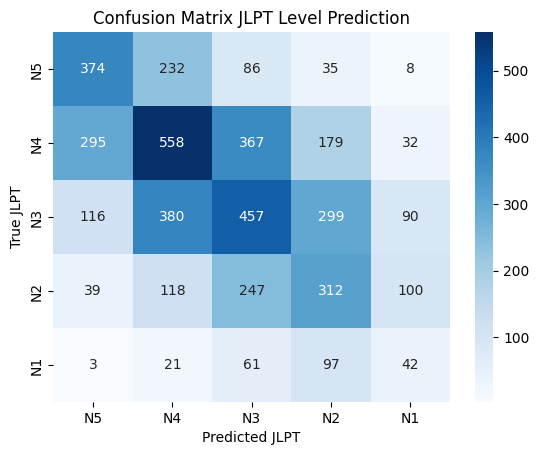
\includegraphics[scale=.4]{img/confusionMatrix}
           \caption[Confusion Matrix for JLPT Level Prediction]{Confusion Matrix for JLPT Level Prediction}
           \label{fig:conMA}
\end{figure}

A common mis-classification was a substantial number of true N3 instances were misclassified as N4(380) or N2 (299).
Similarly, N2 texts were frequently predicted as N3(245) or N1 (107), and N1 texts were often misclassified as N2(
98) or N3(62). This suggests that the model frequently confused text belonging to adjacent proficiency levels,
indicating a high overlap between the proficiency levels. This was confirmed when

This overlap was further supported when aggregating the proficiency levels into broader 3 groups - Beginner (N5+N4),
Intermediate (N3+N2), and
Advanced (N1).
Classification performance for these three groups improved significantly, achieving an overall F1-score of .54. This
substantial increase from .38 F1-score for the five-class problem further corroborates the hypothesis that the
continuous nature of adjacent JLPT levels present a significant challenge for fine-grained classification.

\section{Feature Importance Analysis}
\begin{figure}[h!]
    \centering
    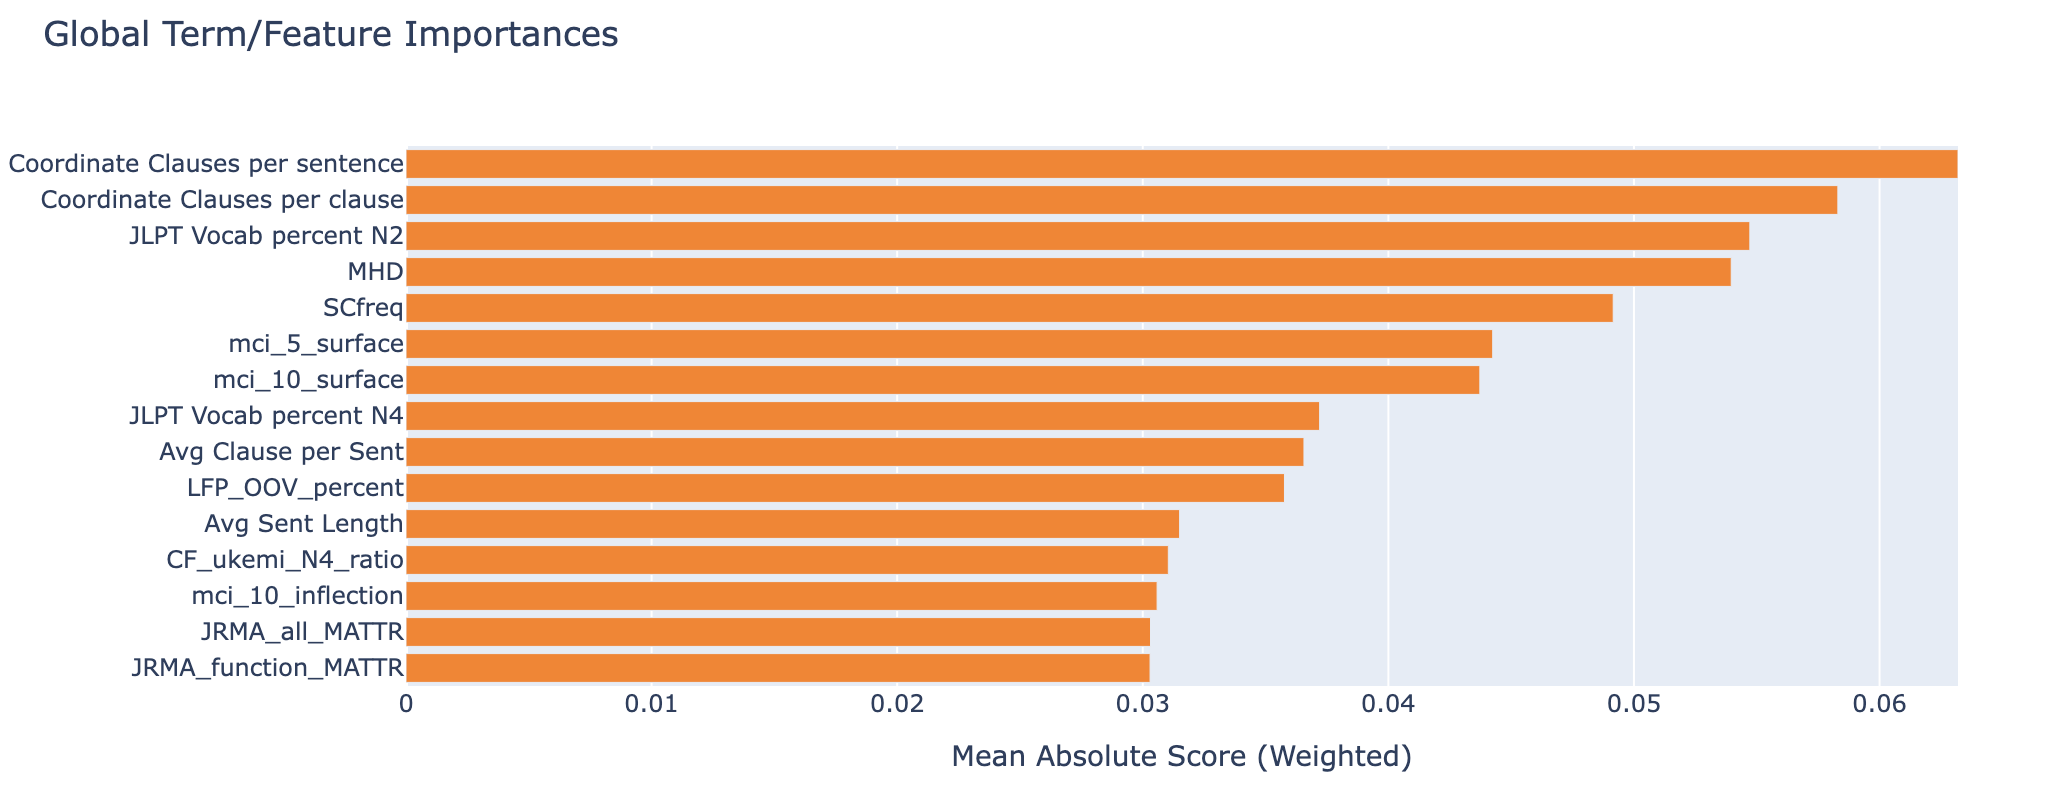
\includegraphics[scale=.4]{img/feature_importance}
    \caption[Feature Importance Chart]{ Feature Importance Chart: Top-ranked features contributing to the classifcation of JLPT proficency levels, based on thier additive contribution scores from the EBM model.}
    \label{fig:featureimportance}
\end{figure}


The feature importance results from the final EBM model are shown in Figure~\ref{fig:featureimportance}. A
more detailed chart showing the top 30 features with weights can be found in Appendix Table~\ref{tab:top30-importance}
Overall, a
diverse range of linguistic features contributed to classification accuracy, though complexity measures were most
prominent among the top-ranked features. A wide variety of complexity
measures consisting of syntactic, lexical and morphological contributed to classification, indicating that a
multidimensional approach is essential for classifying learner texts.

The top two features were coordinate clauses per sentence and coordinate clauses per clause, both measures of
syntactic complexity. These features suggest that the frequency of coordination structures is a strong
differentiator across proficiency levels, potentially a reflection of developmental gains in syntactic elaboration. This
aligns with findings in the previous section, where this feature was also found to discriminate between adjacent
levels in
the low to mid-proficiency ranges while also increasing at higher levels. The class
separation can be seen in Figure~\ref{EBMccPerSent}, where N5 is associated with lower values (below 0.25),
while above 1 are associated with N1 and N2.


\begin{figure}[h!]
    \centering
    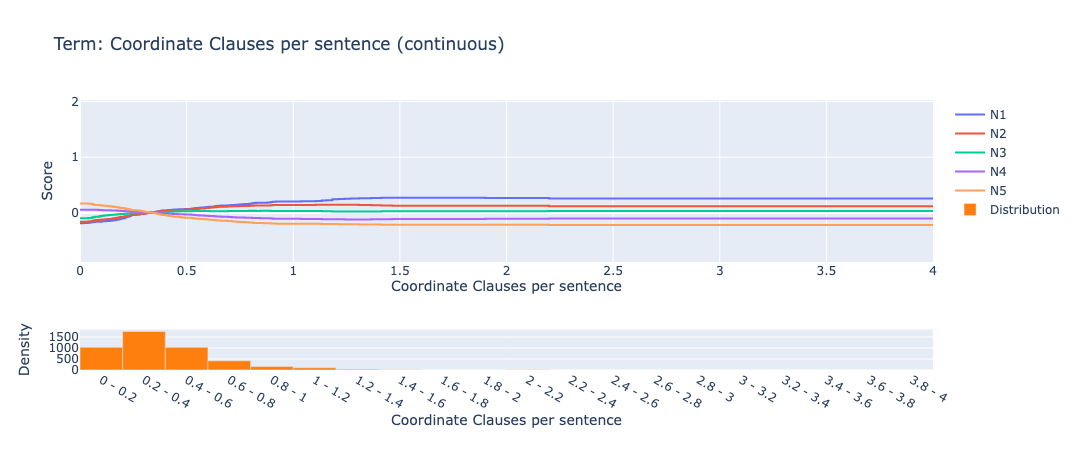
\includegraphics[scale=.4]{img/EBM/EBMccPerSent}
    \caption[Contribution of Coordinate Clauses per Sentence]{This chart represents how the feature of Coordinate clauses per sentence contributes to the prediction of each proficiency level}
    \label{fig:EBMccPerSent}
\end{figure}


The third-ranked feature, the ratio of words from JLPT N2 list to total tokens (Lexical Frequency Profile), highlights
lexical sophistication. A higher proportion of N2-level vocabulary
correlates with higher proficiency levels, consistent with previous lexical profiling studies\citep{Laufer1995}.
As shown in Figure~\ref{fig:EBMjlptN2}, this feature reliably distinguished between the N1 and N2 from the lower
levels.

\begin{figure}[h!]
    \centering
    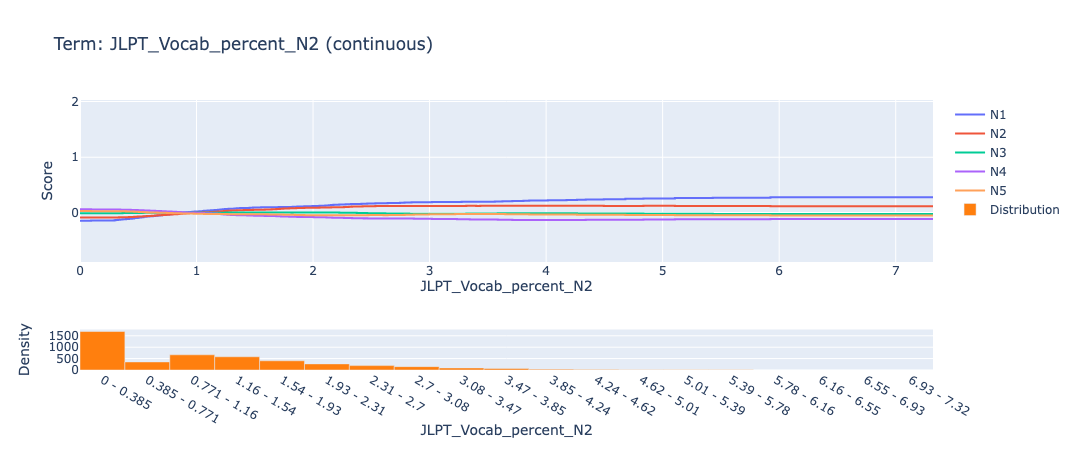
\includegraphics[scale=.4]{img/EBM/JLPTn2P}
    \caption[Contribution of percentage of tokens from JLPT N2 vocabulary list]{This chart shows how the percentage of tokens from JLPT N2 word list contributes to the prediction of each proficiency level}
    \label{fig:EBMjlptN2}
\end{figure}

Mean Hierarchical Distance (MHD), the fourth ranked feature, quantifies the average depth of syntactic embedding.
It's presence in this list suggests that deeper syntactic constructions are a reliable signal to distinguish the
higher proficiency levels.

Subordinate conjunction frequency (SCfreq), a proxy measure for subordination, was ranked fifth. This was somewhat
surprising, as lexical complexity measures such as LFP OOV were expected to be more predictive. However due to the
tokenizer's tendency to misclassify coordinating conjunctions as subordinating ones, SCfreq may effectively capture
both types of clause-linking (coordination and subordination). Since coordination frequency was shown to increase
with proficiency, this blended feature still carries strong predictive value. Figure~\ref{fig:EBMSCfreq} shows its
role in distinguishing N5 from other levels, supported by a broad density range.

\begin{figure}[h!]
    \centering
    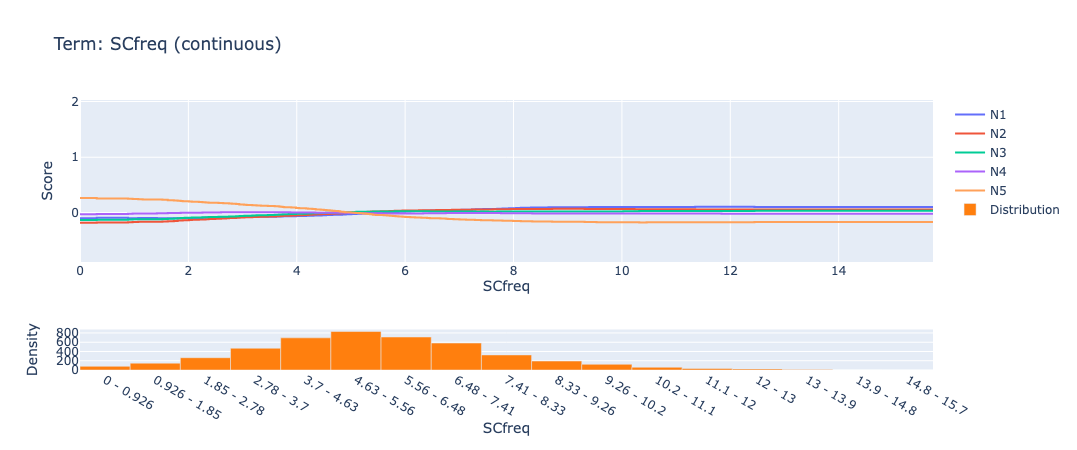
\includegraphics[scale=.4]{img/EBM/EBMSCfreq}
    \caption[Contribution of Subordinating Conjuction Frequency]{This chart shows how feature of Subordinating Conjunction frequency contributes to the prediction of each proficiency level}
    \label{fig:EBMSCfreq}
\end{figure}

Several morphological complexity indicators also appeared in the top features. Both MCI-5 surface and MCI-10
surface were ranked in the top ten, indicating that surface-level morphological diversity increases with
proficiency. Additionally, MCI-10 Inflection, which measures inflectional morphological diversity, as also
influential. This is notewrothy given that the larger text window used in its calculation excluded for shorter
texts. Although previously found to distinguish N1 from a native speaker texts, Figure~\ref{fig:EBMMCI10inflection}
also shows that this feature contributes to differentiating within learner proficiency levels.

\begin{figure}[h!]
    \centering
    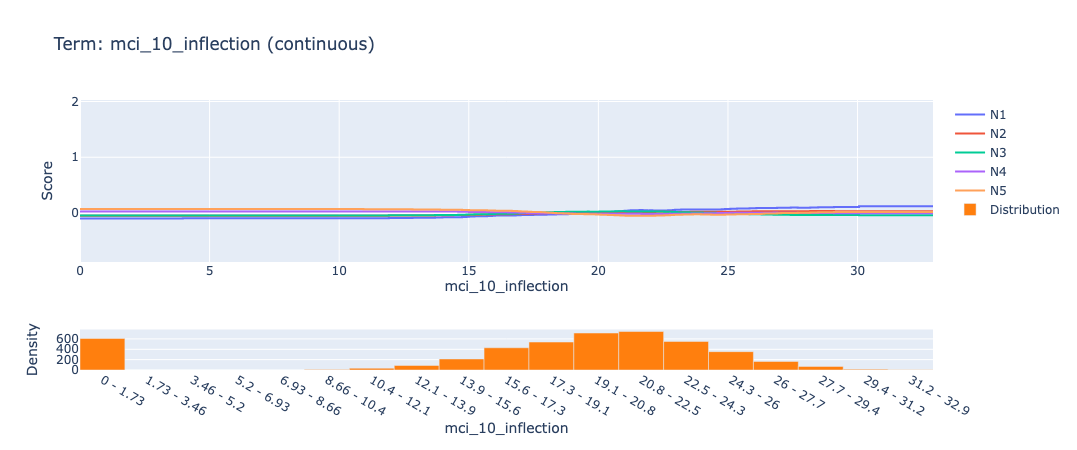
\includegraphics[scale=.4]{img/EBM/MCI10inflection}
    \caption[Contribution of MCI 10 Inflection measure]{This chart shows how the MCI10 inflection measure contributes to the prediction of each proficiency level}
    \label{fig:EBMMCI10inflection}
\end{figure}

JMRA Function MATTR and JMRA All MATTR also ranked within the top 15 as morphological diversity measures. This
suggests that variation in function, and all (function + content) morphemes, which also reflects grammatical
elaboration, is a
relevant factor in distinguishing between proficiency levels. As shown in Figure~\ref{fig:JMRAallMATTR}, higher
All MATTR
scores are associated with the advanced levels (N1 and N2), separating them from lower and intermediate groups.

\begin{figure}[h!]
    \centering
    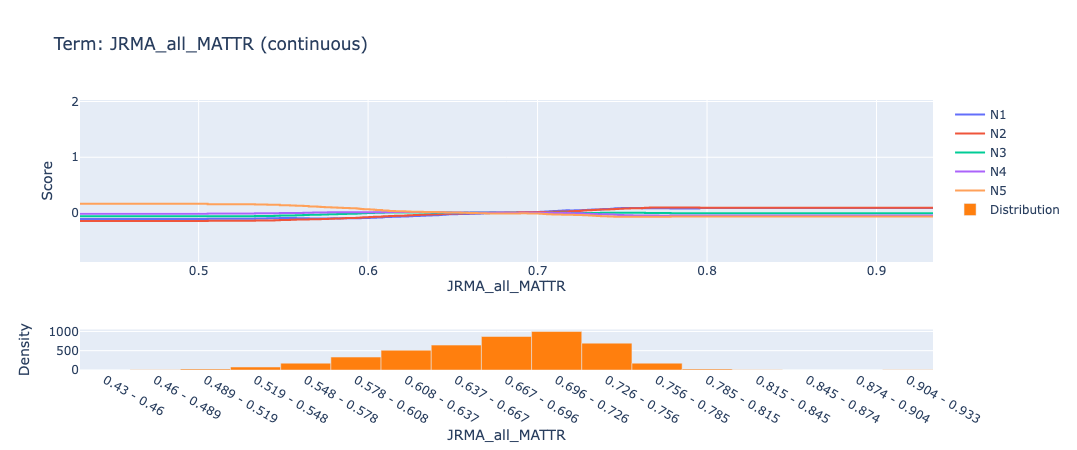
\includegraphics[scale=.4]{img/EBM/JMRAallMATTR}
    \caption[Contribution of JMRA function and content morphemes]{This chart shows how the feature of MATTR of content and function morphemes contributes to the prediction of each proficiency level}
    \label{fig:JMRAallMATTR}
\end{figure}

The proportion of tokens not included in the 10,000 word frequency list of the BCCJW corpus (LFP OOV Percent) was
also highly ranked of importance. This measure of lexical sophistication may signal either the use of advanced
vocabulary or the presence of unrecognized or erroneous forms. As shown in Figure~\ref{fig:EBMlfpOOV}, it
contributed most to distinguishing the lower proficiency levels (N5 and N4), possibly indicating the latter, though
further investigation is needed.


\begin{figure}[h!]
    \centering
    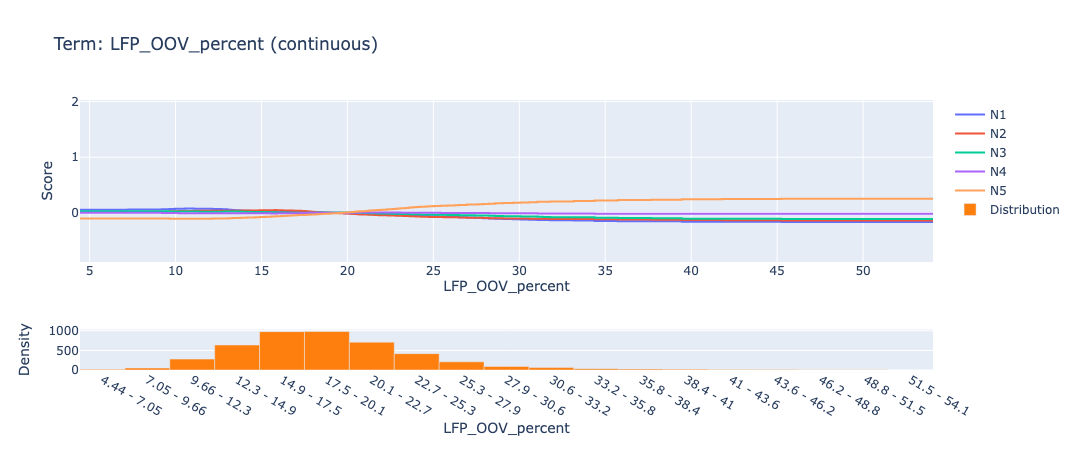
\includegraphics[scale=.4]{img/EBM/EBMlfpOOV}
    \caption[Contribution of Percentage of Lexical Frequency Profile (LFP)Out of Vocabulary (OOV) tokens]{This chart represents how the feature of Lexical Frequency Profile (LFP)Out of Vocabulary (OOV) tokens contributes to the prediction of each proficiency level}
    \label{fig:EBMlfpOOV}
\end{figure}


Only one criterial feature, Ukemi(受身形, passive voice), appeared among the top 15.  Typically introduced to
learners at the N4 level, this form is often difficult to master, due to verb form transformation and unconventional
contexts which may differ from a learner's native language. The highest use of this form was at the N1 level. Figure~\ref{fig:EBMukemi} shows its ability to distinguish between levels, though low overall frequency limits its density and predictive power. Since the extract only captures correct instances incorporating incorrect uses could improve performance.

\begin{figure}[h!]
    \centering
    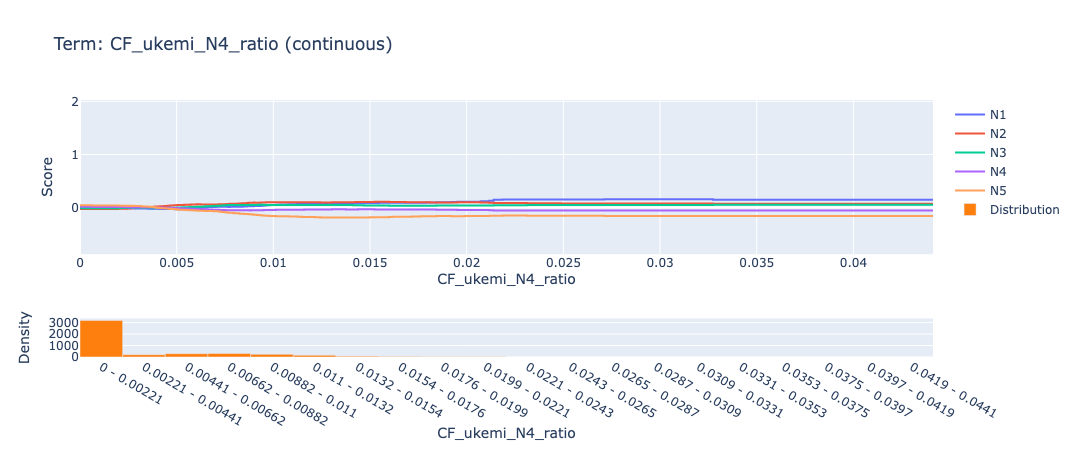
\includegraphics[scale=.4]{img/EBM/EBMukemi}
    \caption[Contribution of ratio of passive form (受身形、ukemi)]{This chart shows how the ratio of passive form to total tokens contributes to the prediction of each proficiency level}
    \label{fig:EBMukemi}
\end{figure}


Unsurprisingly, Sentence length was also among the top features. This was the only measure that consistently
distinguished between all JLPT levels and the native speaker group.

The EBM feature importance analysis confirms that no single metric defines learner proficiency. Rather, a
combination of syntactic elaboration, morphological diversity, and lexical distribution provide the strongest
predictive power.

\section{Discussion}

% Make conrete citations
The results above provide partial support for developmental patterns identified in the previous chapters. In
particular, some features showed a clear trajectory of increased usage of complexity across levels, supporting
earlier corpus based findings and previous literature. However the predictive power of many features was moderate,
as found in the f1 scores, and some expected distinctions between adjacent levels (e.g. N3 vs N2) were not captured
effectively.

This suggests that while form-based measures of grammatical complexity and frequency-based criterial features can be
useful, they may not be sufficient in isolation. Some grammatical forms exhibit nuanced usage that depends on
semantic, pragmatic, or discourse-level factors which are not easily captured through surface-form
analysis alone.

The model's diminished performance, particularly for N2 and N1 as evidenced by lower f1-scores and the high number
of misclassifications in the confusion matrix (Figure~\ref{fig:conMA}), points to inherent challenges in
classifying these adjacent proficiency levels. The significant overlap observed in predictions (e.g. N3 misclassified
as N2 and N4) suggests that the linguistic differences between intermediate and advanced levels are subtler and less
discretely based on the current feature set. It is plausible after all, that learners at adjacent intermediate
levels exhibit similar linguistic characteristics than, for example, a beginner (N5) and an advanced learner (N1).
This continuous nature of language development makes sharp categorical distinctions difficult for any model.

The small sample size of N1 group (44 participants, 224 texts) significantly impacted its classification accuracy (
F1-score
of 0.17 in Table~\ref{tab:trainingResults}). With fewer examples, the model had limited data to learn the specific
criteria that distinguish N1 texts from other levels, leading to a high rate of misclassification, particularly into
N2 and N3 categories. This data imbalance likely constrained the model's ability to fully capture the
characteristics of advanced learners.


\subsection{Limitations and Difficulties}
% integrate limitations from ch 4. into this section:
%One limitation of
%this analysis is that it is purely based on frequency of use and does not capture form-based errors. For forms like the
%passive construction (受身形), which require complex verb transformation and are introduced in later levels, analyzing
%accuracy and types of errors in their production could provide additional insight into learner
%acquisition patterns and developmental stages. Future research should aim to incorporate error analysis to provide a
%more comprehensive understanding of the mastery of grammar features. This would enable a more nuanced understanding
%of not just what forms learners use, but how correctly they use them at different stages of development. Further
%work could also investigate the influence of task genre on the frequency of these grammar forms. This is important
%as certain tasks might elicit specific forms, and understanding this relationship would help refine future corpus
%design attempts to control for these variables and extract specialized forms for more targed analysis.


The corpus, consisting of uncorrected learner language, posed challenges for feature extraction. Misspellings and
grammatical errors common in learner output could lead to incorrect tokenization and POS tagging by the underlying
NLP tools (e.g. SpaCy's Ginza package), thus impacting the accuracy of extracted features. For instance, irregular
forms of "mispellings" might be incorrectly counted as out-of-vocabulary words (in the context of the LFP complexity
measure), rather than as specific error types. More crucially, the morphological complexity of Japanese,
particularly with compound verbs and auxiliary constructions (e.g. 「言い切る」 as one verb vs. 「食べ切る」 parsed into two
parts), meant that rule-based feature extraction struggled with consistency. This could lead to undercounting or
miscategorizing certain complex forms, which are critical indicators of advanced proficiency.

The variability in text length, with some text being very short, likely affected the reliability of certain
density-based metrics, such as MTLD (Mean Type-Token Ratio), if it were included. Such metrics are sensitive to text
length, and calculation over very short texts can yield less stable or representative values, potentially
introducing noise into the feature set.

While features like coordinate clauses per sentence were highly important, the accuracy of their extraction was
dependent on the underlying tokenizer's ability to correctly identify conjunctions and clause boundaries. As noted
previously, many Japanese conjunctions can be used in both coordinating and subordinating contexts, and rule-based
parsers like SpacCy may not fully account for contextual nuances. This potential inaccuracy in the input features
could directly limit the model's ability to use these syntactic measures for precise classification. A more robust,
context-aware parsing system would likely improve the quality of these features.

The feature extractor largely focused on form-based grammatical constructs that are relatively easier to identify
programmatically and are common in standardized written Japanese. This approach may have overlooked more nuanced,
use-based grammatical patterns that could be highly discriminative of proficiency. Futhermore, the reliance on rules
for standardized written language means that variations due to dialects or highly casual written forms, if present
in the learner corpus, would not have been accurately captured, potentially missing valuable information for
classification.

A significant limitation of the current study was the exclusion of learner errors as a direct feature. Different
proficiency levels are often
characterized by distinct error patterns, as was illustrated in \citet{Hawkins_Buttery_2010}.  The
developmental trajectory of errors, where specific error types and frequencies change systematically with
proficiency, could provide highly discriminative information for the model.
Incorporating
systematic error analysis as a
feature
set
could provide
highly discriminative information, potentially leading to substantial improvements in classification accuracy,
especially for distinguishing between adjacent intermediate and advanced levels where subtle error reductions or
shifts in error types might be useful indicators. While these levels have been validated
\citet{jcat_interpretation_guide}, they
are primarily based on recognition tasks (reading and listening) and do not directly assess productive skills like
writing or speaking. Therefore, the proficiency labels assigned to the learner texts, derived from J-Cat, are approximations of a broader construct of proficiency. There can be considerable variance in the productive language capabilities of individuals who score similarly on the JLPT, which might introduce inherent 'noise' or ambiguity into the dataset, further complicating the task of classification for the model.

While EBM demonstrated capability to classify JLPT levels better than chance, performance highlights the inherent
complexity of distinguishing between closely related proficiency levels in a continuous developmental spectrum. The
identified features were significant, but future improvements would benefit from addressing the methodological
challenges in feature extraction, particularly for nuanced Japanese linguistic structures, and exploring the
integration of error-based features. % Results

\chapter{Outlook}
%
% additional research areas/exploration
EGP equivalent for Japanese additional validation of forms used.
% Things that went wrong/were difficult shortfalls

Ideas: explore-accommodation for the third domain - Fluency (possibly using timing??)  Focus on Accuracy together...

More accurate analysis of clauses needed to answer additional questions about development of clausal complexity

This tool could also be useful for approximating the JLPT level a learner should take.

better analysis of てform? i.e. coordinate clauses, it is included in the grammar forms connected with other parts
but not on its own. The use of てform most likely makes up a good percentage of the coordinate clauses. (even through
the て is marked as SCONJ) % Outlook


%% ----------------------------------------------------------------
% Now begin the Appendices, including them as separate files

\addtocontents{toc}{\vspace{2em}} % Add a gap in the Contents, for aesthetics

\appendix % Cue to tell LaTeX that the following 'chapters' are Appendices

\chapter{An Appendix}

list of measures (I will make this pretty later)
Syntactic Complexity
\begin{itemize}
    \item Sentence Length
    \item Clause Length
    \item Clauses per sentence
    \item Coordinate Clauses per sentence
    \item Coordinate Clauses ratio to all clauses
    \item Subordinate Clauses per sentence
    \item Subordinate Clause Ratio to all clauses
    \item Subordinate Clauses to Coordinating Clauses
    \item Average Noun Phrase length
    \item Average Verb Phrase Length
\end{itemize}

Lexical Complexity
\begin{itemize}
    \item Corrected Type Token Ratio
    \item Average word length
    \item Noun Density
    \item Verb Density (including auxilaries)
    \item Adjective Density
    \item Adverb Density
    \item MTLD
    \item Lexical Frequency Profile
\end{itemize}

Morphological Complexity
\begin{itemize}
    \item MCI - 5
    \item MCI - 10
    \item KOMORA (MATTR and MTLD)
\end{itemize}

Discourse
\begin{itemize}
    \item -
\end{itemize}

Semantic
\begin{itemize}
    \item - will not implement
\end{itemize}

Cohesion/Coherence
\begin{itemize}
\end{itemize}


Criterial Features
\begin{table}[h!]
\centering
\begin{tabular}{lll}
\hline \textbf{JLPT Proficiency Level} & \textbf{Grammar Form} & textbf{English Equivalent}  \\ \hline

N1  &	あえて &	        dare to \\
N1  &	案の定 &	        just as one thought\\
N1  &	あらかじめ   &	beforehand; in advance\\
N1  &	ばこそ &	        only because\\
N1  &	どうにも○○ない    &	not … by any means\\
N1  &	ほうがましだ  &	I would rather\\
N1  &	いかなる	&       any kind of\\
N1	&   可能性がある  &	there's a possibility\\
N1	&   かつて	&       once; before\\
N1	&   嫌いがある &     	to have a tendency to\\
N1	&   きりがない	&   there's no end to\\
N1	&   もしくは	    &   or; otherwise\\
N1	&   てみせる	    &   I'll definitely\\
N1	&   てしかるべきだ & 	should\\
N1	&   という     &   	all; every\\
N1	&   とは	    &       (indicates word or phrase being defined); or expression of surprisal\\
N1  &	とはいえ	&       nonetheless; although\\
N4	&   以上  	&       over\\
N2	&   以上に	&       more than; no less than\\
N2	&   えない    &     	unable to; cannot\\
N2	&   える / うる &	can; is possible\\
N2	&   お○○願う &     	could you please\\
N2	&   恐れがある &     	there are fears that\\
N2	&   かいがある &     	it's worth one's effort to do something\\
N2	&   限り	        &   as long as; while… is the case\\
N2	&   かと思ったら / かと思うと	& then again; just when; no sooner than\\
N2	&   から言うと   &	in terms of; from the point of view of\\
N2	&   からして	&   judging from; based on\\
N2	&   からすると / からすれば	&   judging from; considering\\
N3	&   さらに    &   	furthermore; again; more and more\\
N2	&   しかも	&       moreover; furthermore\\
N2	&   次第	     &      as soon as\\
N2	&   次第だ / 次第で &	depending on; so\\
N2	&   その上	&       besides; in addition; furthermore\\
N3	&   それとも  &	    or; or else\\
N2	&   それにしても & 	nevertheless; even so\\
N3	&   だけでなく   &	not only… but also\\
N2	&   つつ	&           while; although\\
N3	&   つもりで	&       with the intention of doing\\
N2	&   でしかない	&   merely; nothing but; no more than\\
N3	&   てしょうがない & 	very; extremely\\
N2	&   てたまらない	&   very; extremely; can't help but do\\
N2	&   て当然だ	&       natural; as a matter of course\\
N2	&   てはいられない & 	can't afford to; unable to\\
N2	&   というものだ  &	something like…; something called…\\
N2	&   と考えられる &	one can think that…\\
N3	&   ないことにはない &	states something is not quite impossible but requires great effort\\
N2	&   ないではいられない & can't help but feel; can't help but do\\
N2	&   なお	    &        furthermore; still; yet (used to add more information to the )\\
N2	&   にかかわらず &	regardless of\\
N2	&   に限って &	    only; particularly when\\
N2	&   に限らず &	    not just; not only… but also\\
N2	&   に限る &       	nothing better than; there's nothing like\\
N2	&   に決まっている &	I'm sure that…\\
N2	&   に応えて	    &   in response to\\
N2	&   に基づいて   &   	based on\\
N2	&   に過ぎない	&   no more than; just; merely\\
N2	&   にもかかわらず &	despite; in spite of; although\\
N2	&   ねばならない  &	have to; must\\
N2	&   果たして    &  	sure enough; really\\
N2	&   ふうに	&       in a way (this way/that way/what way)\\
N3	&   ぶりに	&       for the first time in\\
N3	&   むしろ	&       rather; instead\\
N2	&   もかまわず   &	without worrying about\\
N2	&   もっとも    &	but then; although\\
N2	&   ものがある &     	(sentence-ending expression of strong judgement)\\
N2	&   ものだから   &	because; the reason is\\
N2	&   ものの      &   	but; although\\
N2	&   やがて &       	soon; before long; eventually\\
N2	&   やら○○やら  &	such things as\\
N2	&   よりほかない  &	to have no choice but\\
N3	&   あまり     &   	so much… that \\
N3	&   あまりに    &	so much… that; too…\\
N3	&   いくら○○ても / いくら○○でも   &	no matter how\\
N3	&   一方だ	    &   more and more; continue to \\
N2	&   一方で	&   on one hand; on the other hand は優しい。\\
N3	&   うちに &   	while; before; doing \\
N3	&   おかげで &	thanks to; because of \\
N3	&   がたい &   	hard to; difficult to\\
N3	&   ぎみ  &   	-like; -looking\\
N3	&   きる  &	    to do something completely\\
N3	&   切れない	 &  being too much to finish\\
N3	&   くせに &   	even though; and yet; despite\\
N3	&   決して○○ない &	never; by no means \\
N3	&   こそ	    &   certainly (emphasises the previous word)\\
N4	&   ことがある   &	can; sometimes happens\\
N3	&   ことはない   &	there is no need to; never happens\\
N3	&   さえ	    &   even  \\
N3	&   しかない    &	have no choice but\\
N3	&   ずに  &   	without (doing) \\
N3	&   せいで &   	because of  \\
N3	&   だけど &   	but; however\\
N3	&   確かに &	    surely; certainly\\
N3	&   たびに &   	everytime; whenever\\
N3	&   ついでに   &	taking the opportunity; while (you) are at it\\
N3	&   っぱなし  &	    leaving something still in use\\
N3	&   っぽい &   	    -ish; -like \\
N3	&   つまり &   	    in other words; that is to say\\
N4	&   という &   	    called; named\\
N3	&   というより  &    rather than\\
N3	&   と共に &   	    together with\\
N3	&   とは限らない &	not necessarily so; is not always true\\
N3	&   ながら / いながら / ながらも	&   although; despite \\
N3	&   なぜなら / なぜかというと  &	because; the reason is\\
N3	&   なるべく    &	as much as possible\\
N3	&   に比べて	&       compared to\\
N3	&   に違いない   &	I'm sure; no doubt that\\
N3	&   ばよかった   &	should have; it would have been better if\\
N3	&   べき       &   	must do; should do\\
N3	&   ほど	    &       the more; to the extent that; so much… that\\
N3	&   もしかしたら  &	perhaps; maybe\\
N3	&   ような気がする &	have a feeling that; think that\\
N4	&   受身形 &        Passive Form\\
N4	&   あまり○○ない &	not very; not much\\
N4	&   かしら &       	I wonder\\
N4	&   がする &       	smell; hear; taste\\
N4	&   かもしれない  &	might; maybe\\
N4	&   ございます   &	there is (honorific ある)\\
N4	&   させられる   &	to be made to do something\\
N4	&   させる &       	to make/let somebody do something\\
N4	&   しか○○ない &	    only; nothing but\\
N5	&   すぎる     &   	too much\\
N4	&   たところ    &   	just finished doing; was just doing\\
N4	&   たばかり    &   	just did; something just happened\\
N4	&   たら  &       	if; after; when\\
N4	&   たらどう    &	why don't you\\
N5	&   たり○○たり  &	do such things like\\
N4	&   ていただけませんか&	could you please\\
N4	&   ているところ  &	in the process of doing\\
N4	&   てくれる    &	to do something for someone \\
N4	&   てしまう / ちゃう  &	to do something (regretfully); to do something (completely) \\
N4	&   てすみません  &	I'm sorry for\\
N4	&   てもらう    &	to get somebody to do something\\
N4	&   と思う &       	I think; you think\\
N4	&   ところ     &   	about to; on the verge of\\
N5	&   なくてはいけない / なくてはならない &	must do; have to do\\
N4	&   なさい	&       order somebody to do something\\
N4	&   なさる &       	to do (honorific する) \\
N4	&   にくい     &   	difficult to\\
N4	&   のように / のような &	like; similar to\\
N4	&   みたい &       	like; similar to; resembling\\
N4	&   みたいに/みたいな   &	like; similar to\\
N4	&   やすい &       	easy to; likely to\\
N4	&   ようだ &       	it seems that; it appears that; it looks like\\
N4  &	より  &       	than\\
N4	&   られる1    &   	to be able to do something\\
N4	&   られる2    &   	to do (by someone) (passive 受身形)\\
N5	&   いちばん    &	the most \\
N3	&   くらい / ぐらい   &	about; approximately\\
N5	&   たい  &	want to\\
N5	&   つもり &	plan to; intend to\\
N5	&   てください   &	please do…\\
N5	&   ほうがいい   &	it'd be better to, state a preference\\
N5	&   ほうがいい2  &   	it'd be better to not\\





\hline
\end{tabular}
\caption[Proficency Levels]{JLPT proficency level classification based on J-cat score ranges, adapted from
\cite{jcat_interpretation_guide}.}
\label{tab:proficency-table}
\end{table}

Also list the features/forms I am including in my analysis	% Appendix Title

%\input{Appendices/AppendixB} % Appendix Title

%\input{Appendices/AppendixC} % Appendix Title

\addtocontents{toc}{\vspace{2em}}  % Add a gap in the Contents, for aesthetics
\backmatter

%% ----------------------------------------------------------------
\label{Bibliography}
\lhead{\emph{Bibliography}}  % Change the left side page header to "Bibliography"
\bibliographystyle{acl_natbib}  % Use the "unsrtnat" BibTeX style for formatting the Bibliography
\bibliography{Bibliography}  % The references (bibliography) information are stored in the file named "Bibliography.bib"

\end{document}  % The End
%% ----------------------------------------------------------------